%\chapter{Real Data}
%Finally, we also performed inference on a real FMRI scan. The scanner we used...
%... more specifics...

% TODO include single?
%Before performing tests on a full image, I the particle filter
%on regions deemed active and inactive by statistical parametric mapping
%(SPM). This served the purpose of adjusting the priors as well as the 
%preprocessing based on real world signals. This was actually done before
%the simulations, and then results were carried back the simulations 
%to check consistency.
%After work adjusting parameters, most importantly the weighting function and the 
%priors, particle filter was applied to every voxel in an FMRI image.
%The results of this large scale analysis was a parameter map which was
%then used to calculate normalized square-root MSE image. 
%
%\section{Single-Voxel Analysis}
%The choice of a prior, as discussed previously, is extremely important. While a
%prior may have the potential to give good results, being a monte-carlo algorithm
%there is the possibility for inconsistencies. Thus, increasing the variance
%of the time-constants may allow additional flexibility, it will also cause
%additional model variance. Before running on a full volume I adjusted the 
%prior to ensure that the same input would give the same output 100 times in a 
%row. While this may seem like a given, with a random drawing of the prior,
%this can be difficult. Case in point, the exact same algorithm run twice
%with the time constants all having standard deviations of $.35$ resulted in two
%very different fits, shown in \autoref{fig:badfit_param1}.
%
%\begin{figure}
%\subfigure{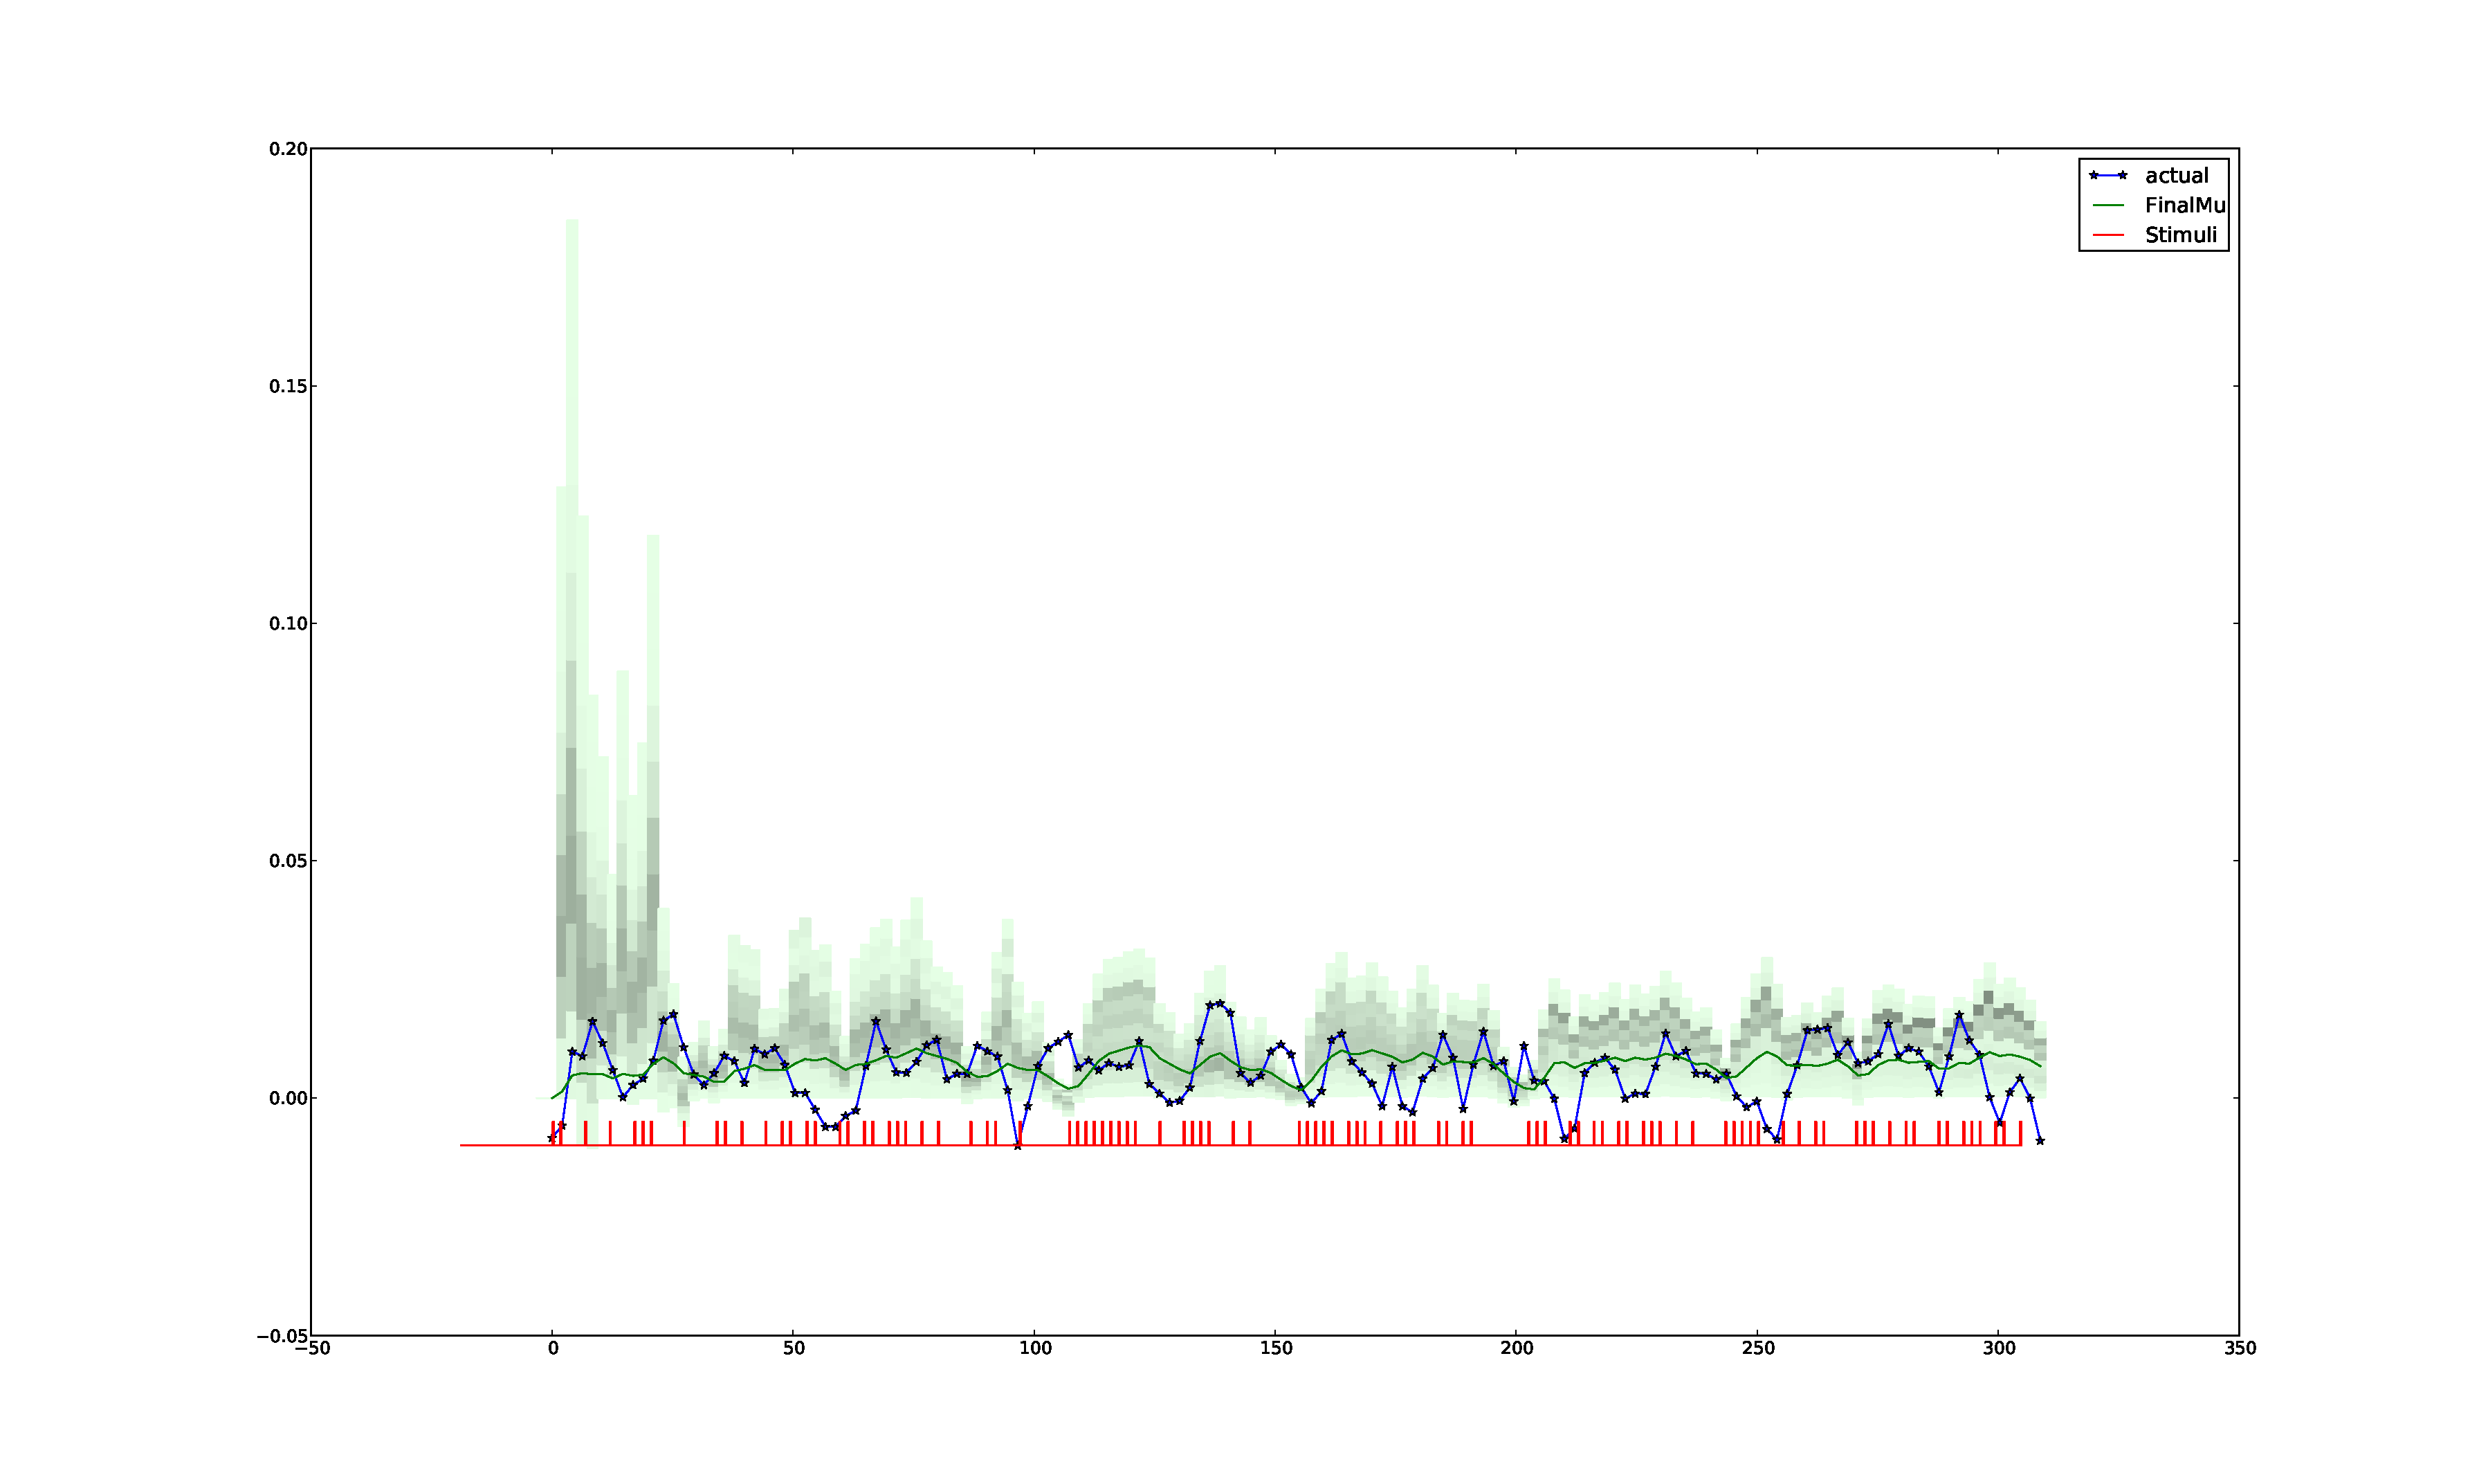
\includegraphics[clip=true,trim=6cm 2cm 6cm 3.5cm,width=17cm]{images/badfit_param1}}
%\subfigure{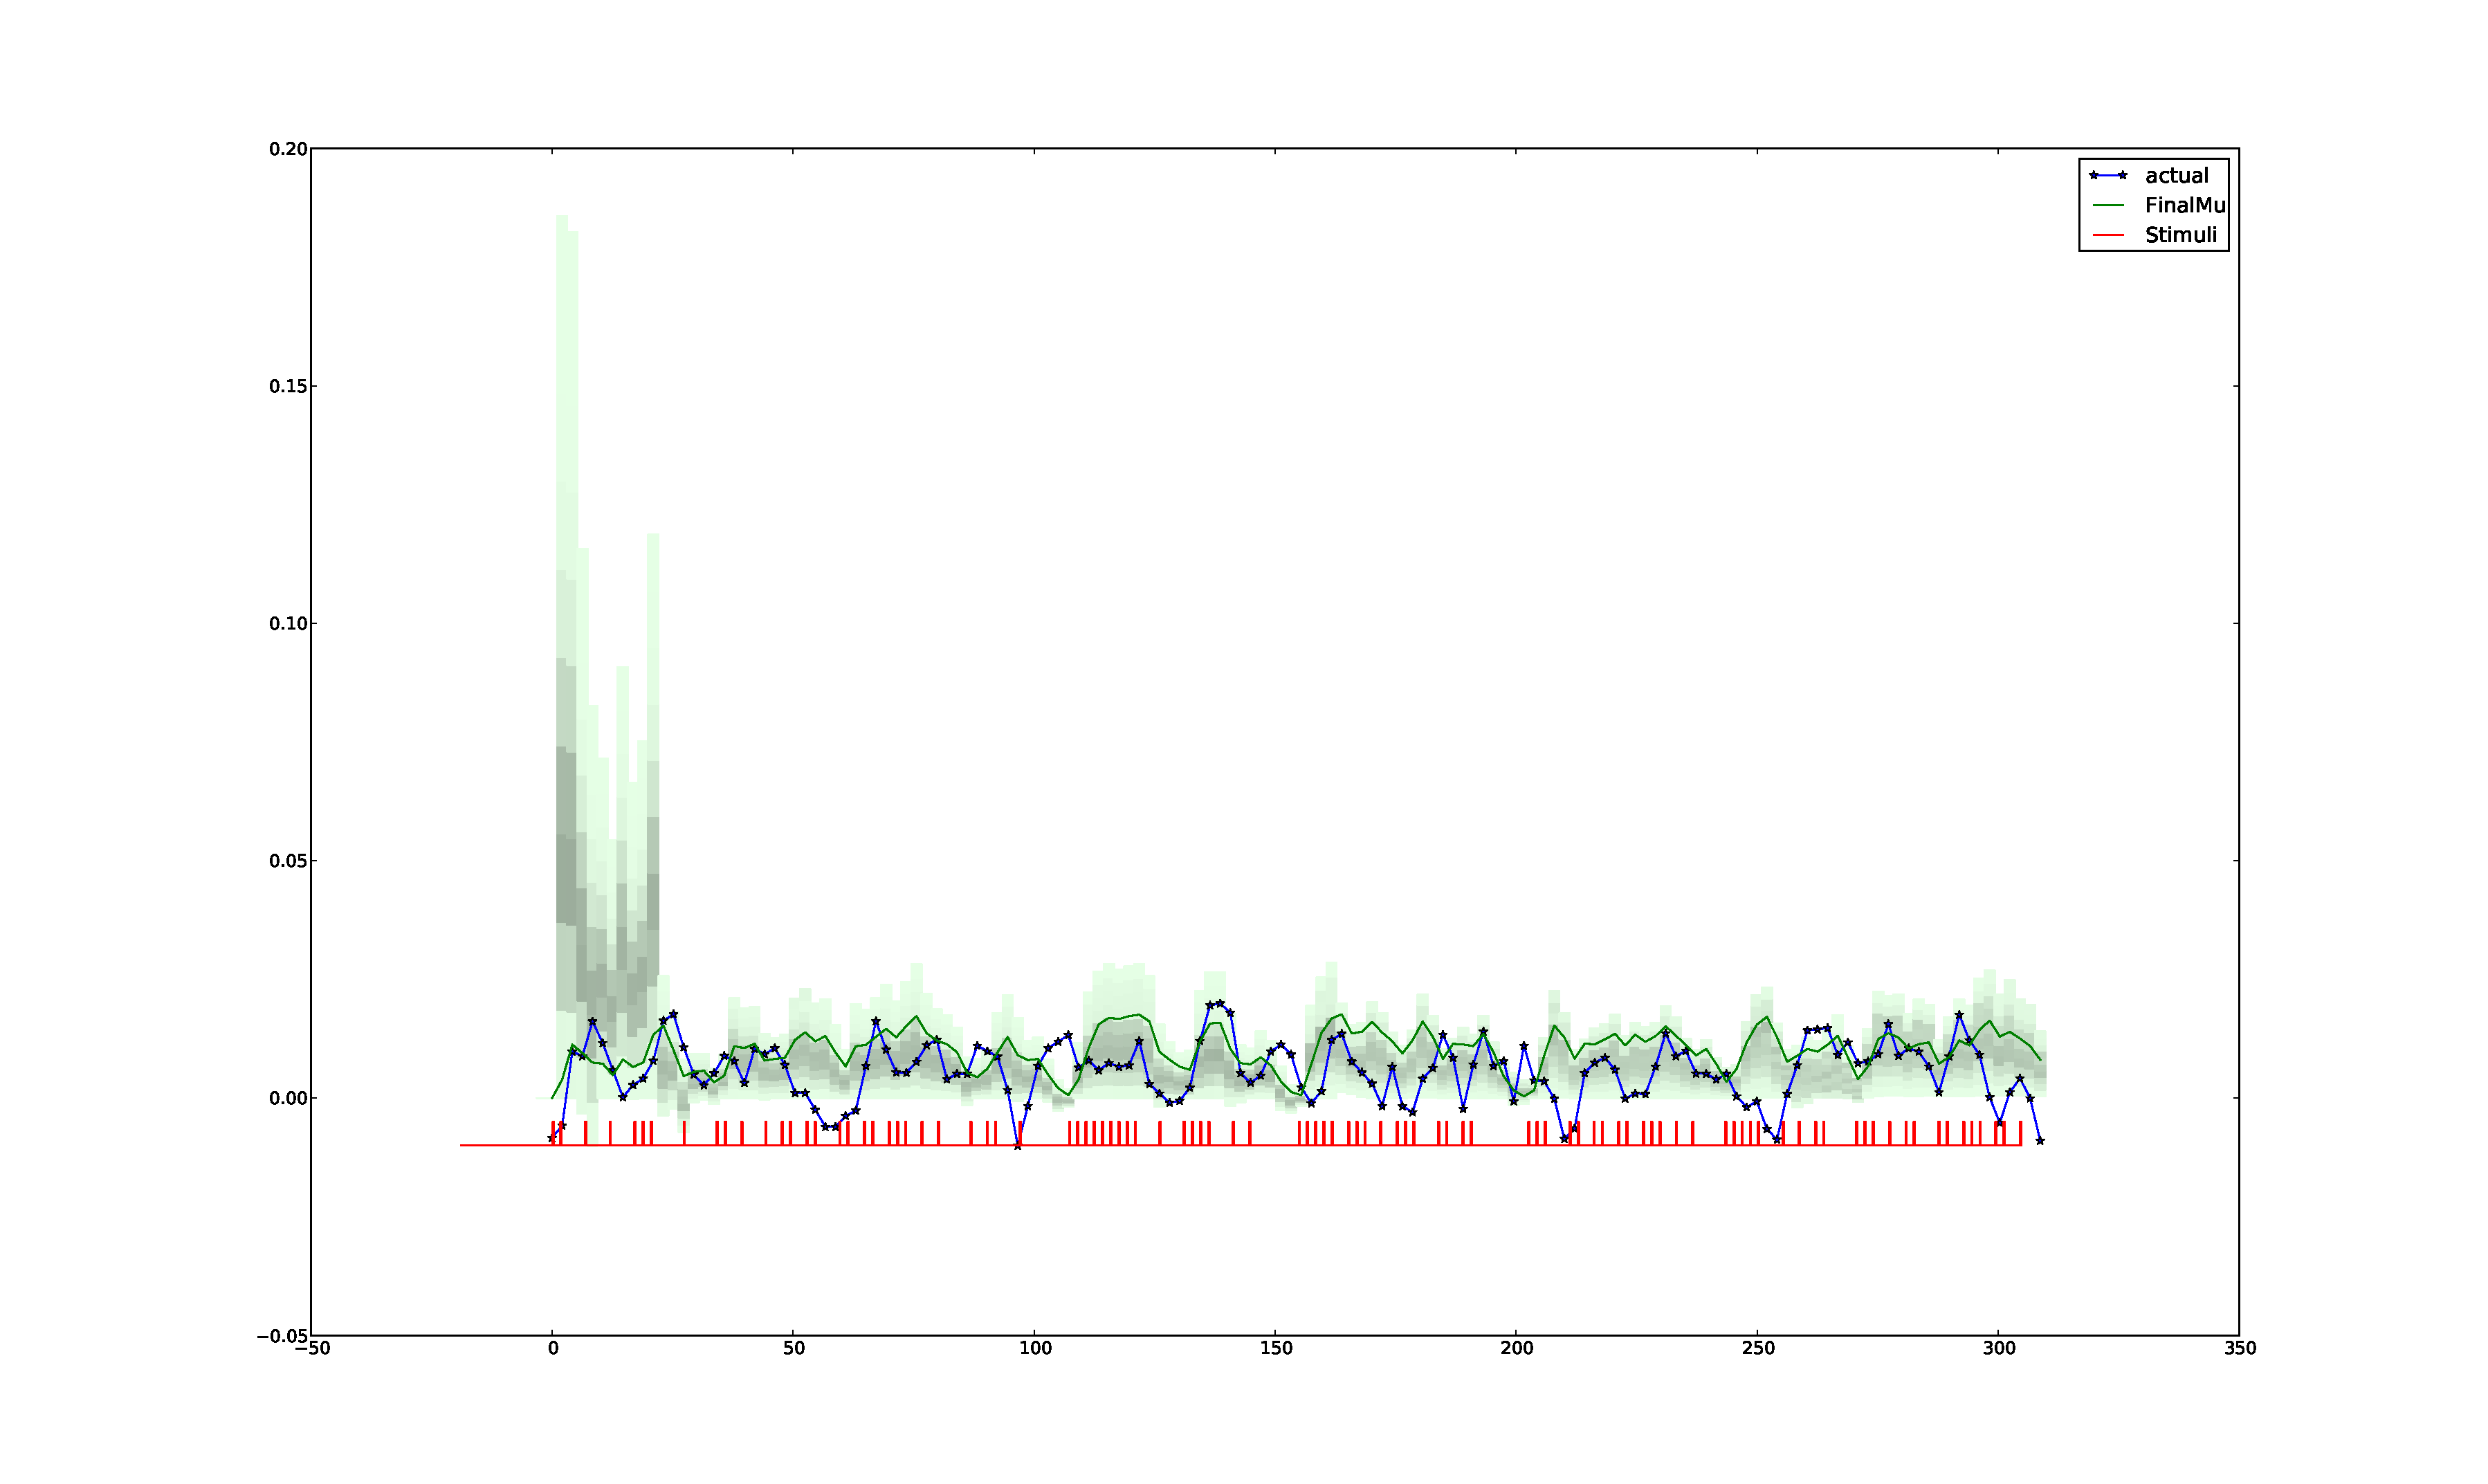
\includegraphics[clip=true,trim=6cm 2cm 6cm 3.5cm,width=17cm]{images/goodfit_param1}}
%\caption{The same priors gave rise to both fits.}
%\label{fig:badfit_param1}
%\end{figure}
%
%For this reason, I actually lowered the standard deviations of the time
%constants to prevent over-smoothing. This resulted in more consistent,
%though potentially slightly worse fits, two examples of which are 
%shown in \autoref{fig:param2_var}. 
%
%\begin{figure}
%\subfigure{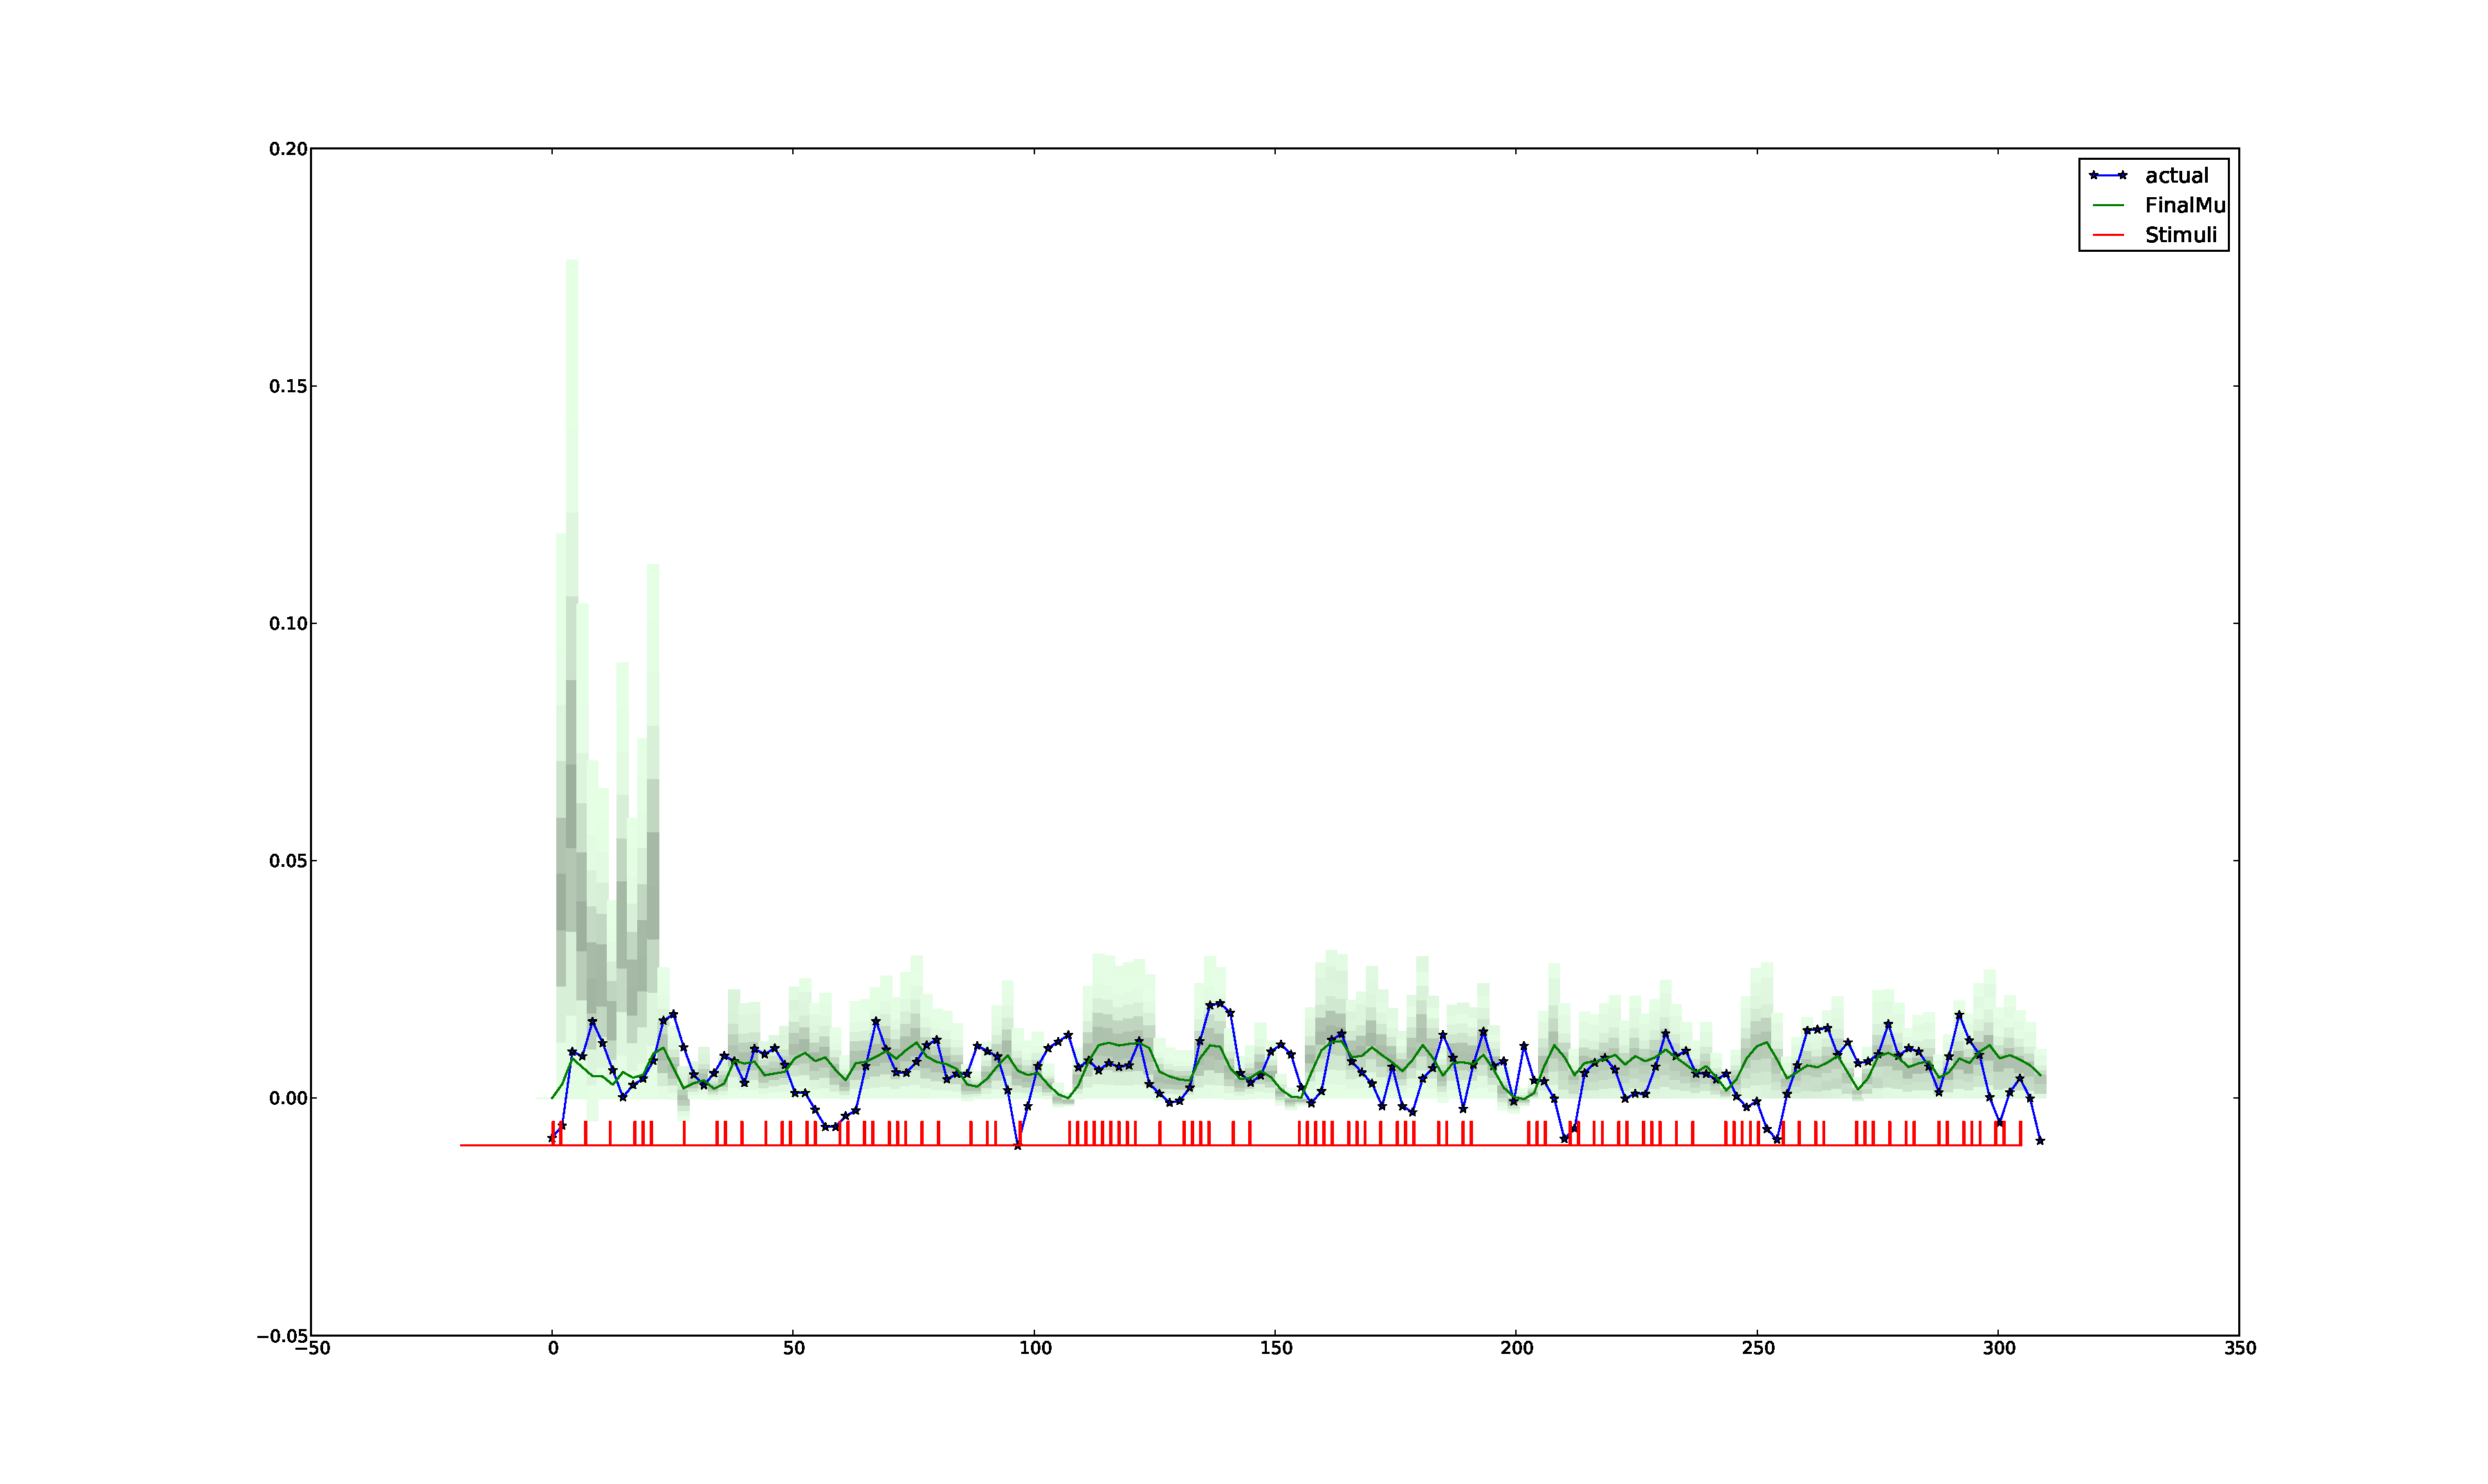
\includegraphics[clip=true,trim=6cm 2cm 6cm 3.5cm,width=17cm]{images/param2a}}
%\subfigure{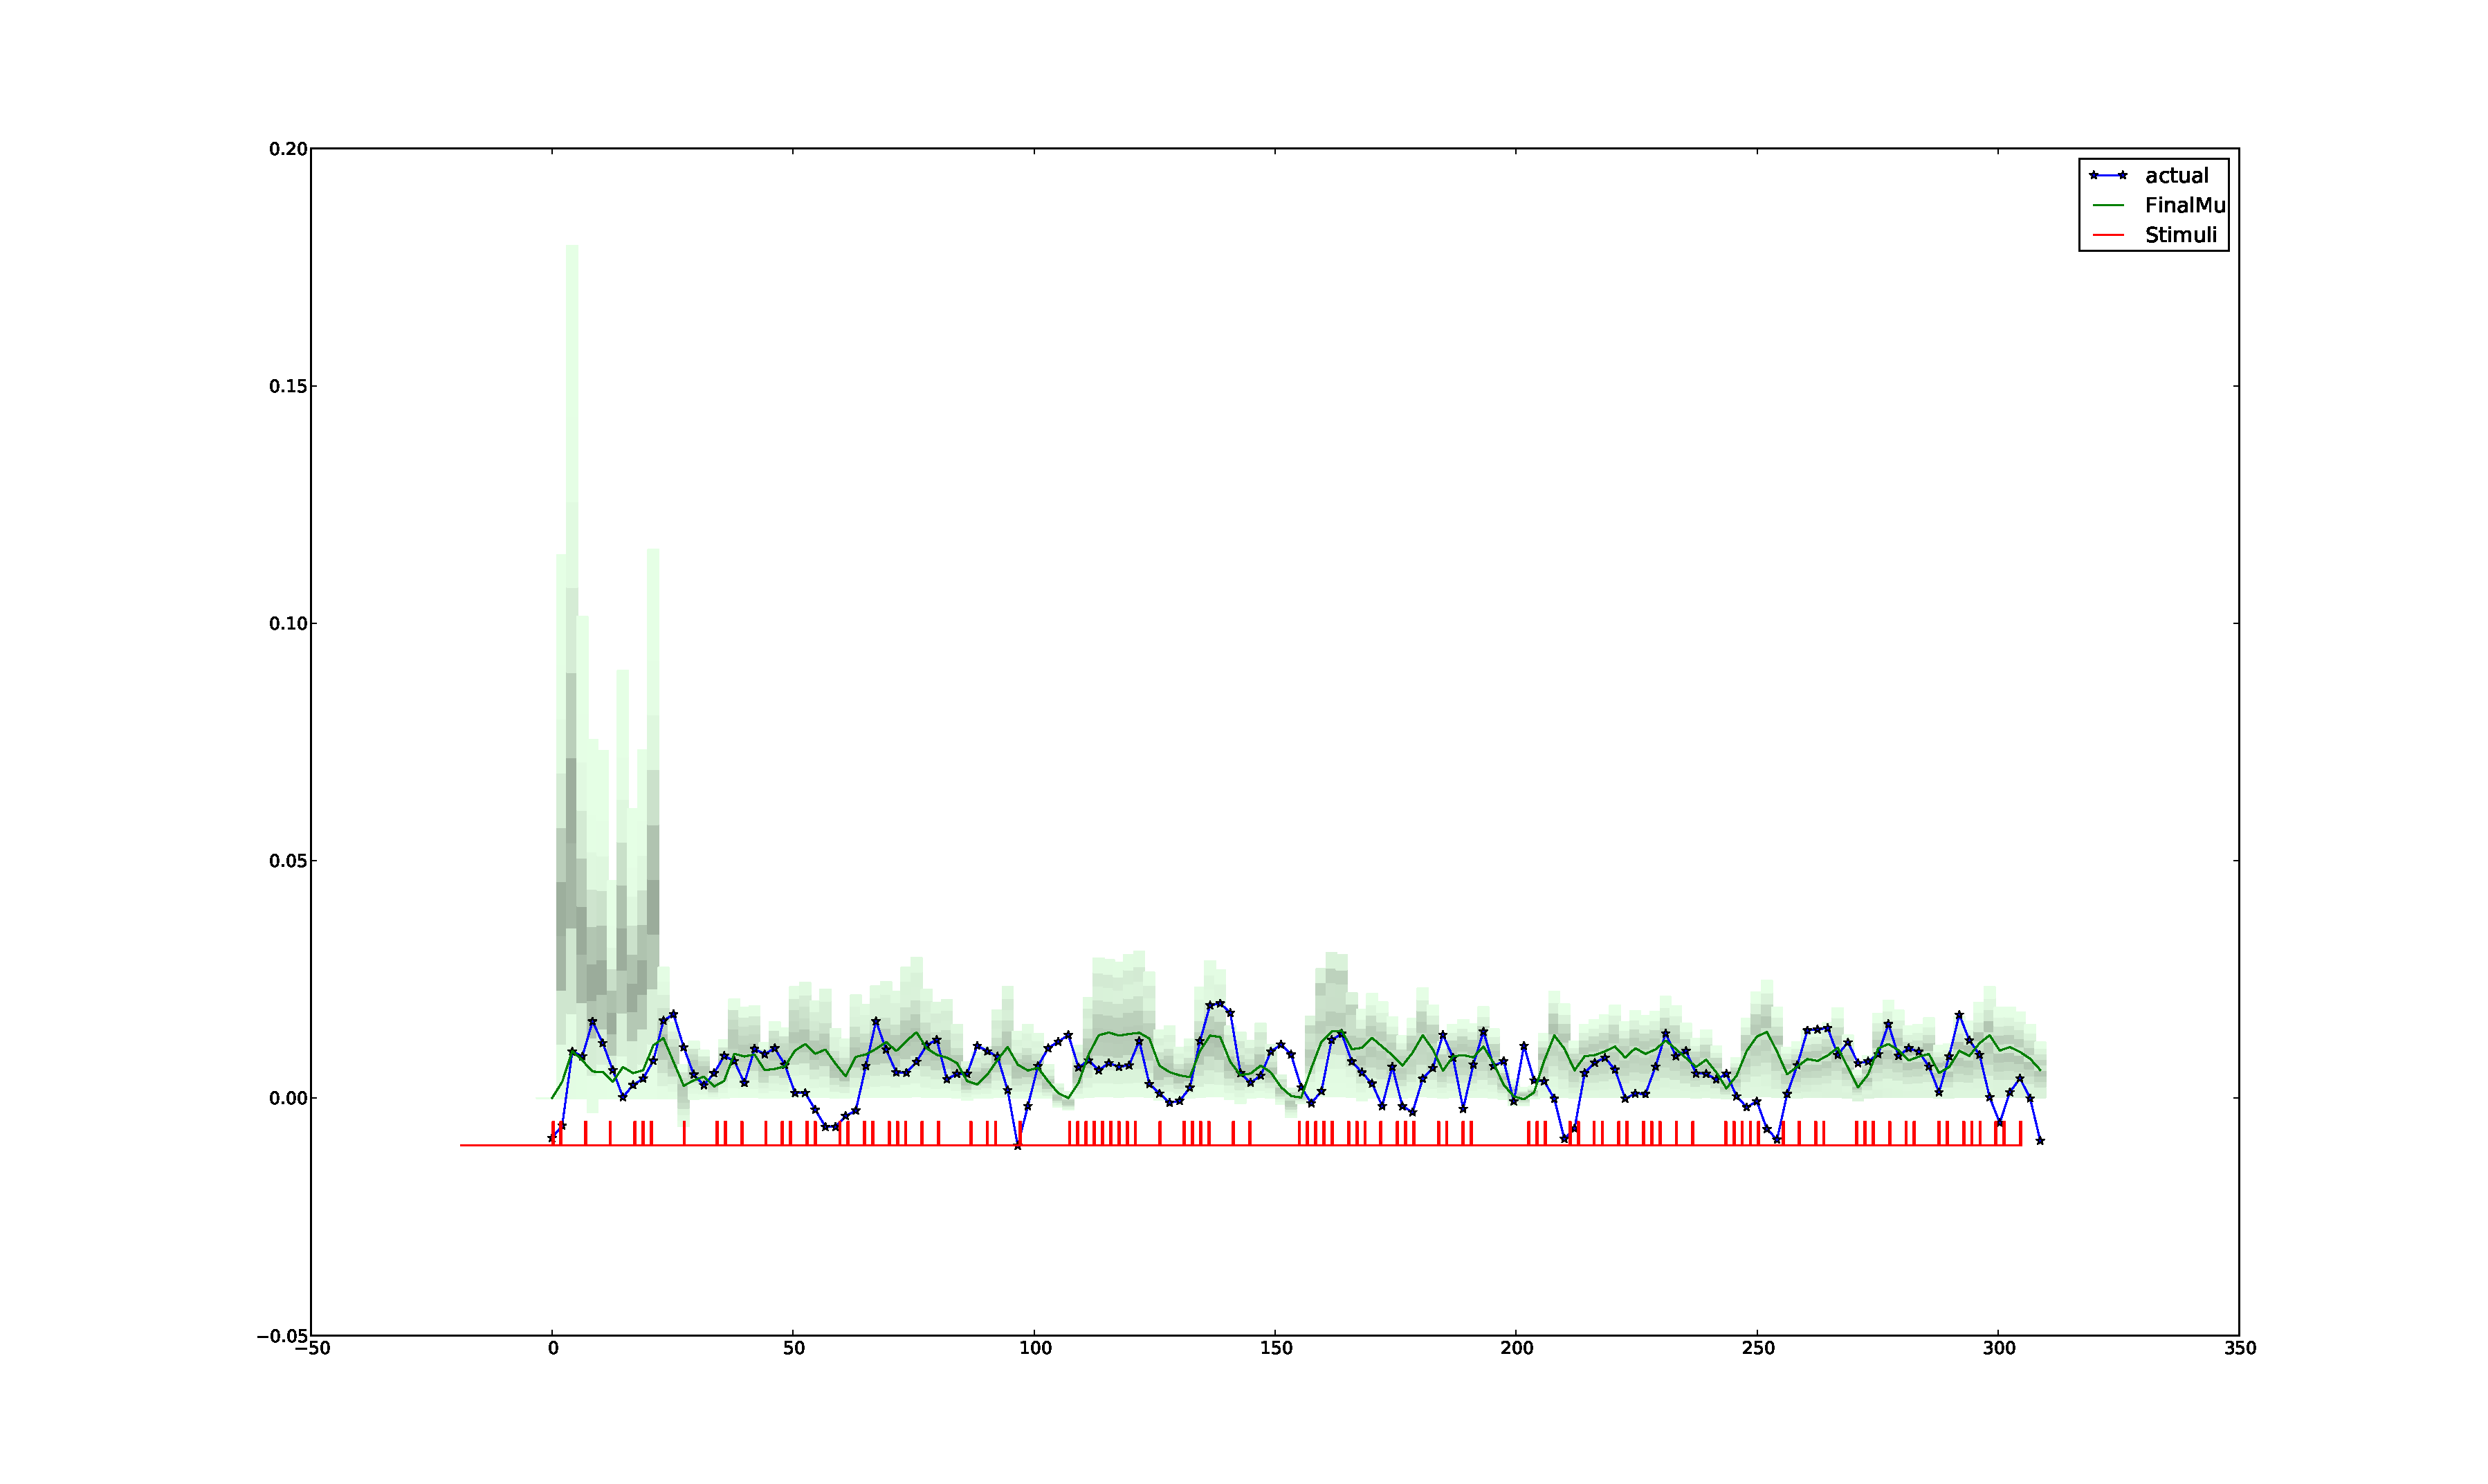
\includegraphics[clip=true,trim=6cm 2cm 6cm 3.5cm,width=17cm]{images/param2b}}
%\caption{A poor fit, using the same parameters as }
%\label{fig:param2_var}
%\end{figure}
%
%todo: stats of the 100 fits?
%
%\section{Single Time-Series Simulation}
%
\chapter{Real Data}
\label{sec:RealData}
Modeling the BOLD response is of course not of much use if it is only done in a 
single voxel. Although this algorithm will hopefully lead to more novel methods 
of analysis, the standard use for modeling the BOLD signal is to locate "activation".
By activation I really mean areas where the input correlates with the BOLD response, 
thus indicating that the stimuli is driving some sort of neural activity. Of course 
much more is going on behind the scenes, brain regions are stimulating other brain
regions, but before that can be analyzed we must validate the ability of the particle
filter to be able to accurately find and model activation. Once areas where the BOLD 
model may be accurately estimated are found, integrating the model will allow for accurate
simulation between measurements, which then may be used for more advanced analysis.
Again though, it all begins with localizing the first activation regions in the
chain. Therefore here I compare the output of the particle filter based modeling
solution to the conventional SPM method. 

In reality, the SPM8 method is a different animal from the algorithm described here.
First SPM preprocesses the image by spatially smoothing the FMRI image (here with 
an $8mm x 8mm x 8mm$ Gaussian kernel), whereas
this is not done in the particle filter algorithm. Additionally, a spline
is used to de-trend, rather than SPM8's high pass filter with a cut
off based on a globally estimated autocorrelation. Thus the preprocessing pipelines 
are different, and the output of SPM8 is single t-statistic, whereas the output 
of the particle filter is a posterior probability distribution of the parameters
at every single voxel. To validate the quality of the particle filter results though
it is necessary to compare the location of
"activated" voxels, and the goodness of fit provided by each method. 

The results from SPM8 are shown in \autoref{fig:hm_canon_spm}, and the results from 
the particle filter are shown in \autoref{hm_canon_pfilter}.

\begin{figure}
\subfigure[]{\label{fig:hm_spm} 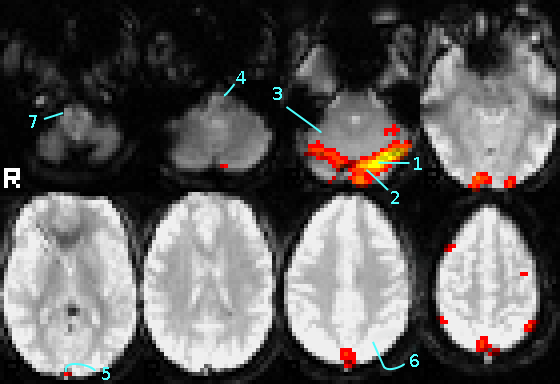
\includegraphics[scale=.66]{images/spm_hm}}
\subfigure[]{\label{fig:hm_canon_spm_x} 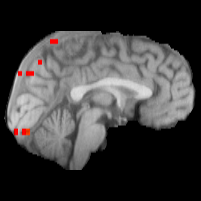
\includegraphics[scale=.85]{images/spm_hm_x}}
\subfigure[]{\label{fig:hm_canon_spm_y} 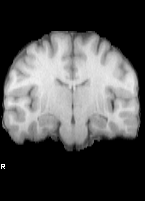
\includegraphics[scale=.85]{images/spm_hm_y}}
\subfigure[]{\label{fig:hm_canon_spm_z} 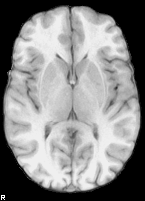
\includegraphics[scale=.85]{images/spm_hm_z}}
\subfigure{\label{fig:scale_spm} 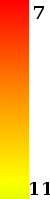
\includegraphics[scale=.3]{images/scale1}}
\caption{Sagittal, coronal and axial slices of SPM results (\autoref{fig:hm_canon_spm_x} \autoref{fig:hm_canon_spm_y} 
         \autoref{fig:hm_canon_spm_x}), as well as a series of axial slices, \autoref{fig:hm_spm}. Units
         of activation are in Student's T-scores. Higher indicates higher assurance that the signal cannot
         have occurred through noise alone.}
\label{fig:hm_canon_spm}
\end{figure}

\begin{figure}
\subfigure[]{\label{fig:hm_pfilter} 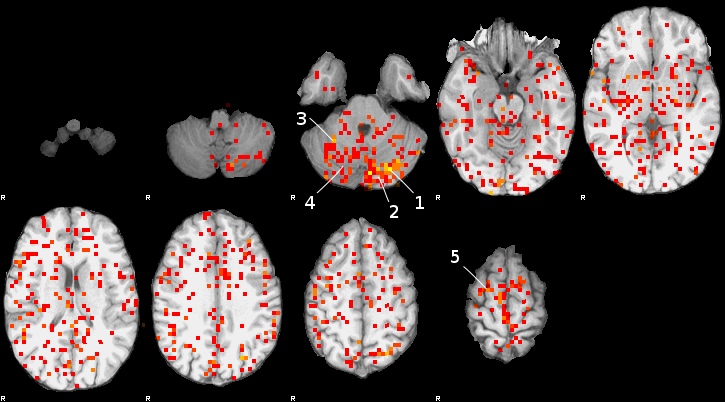
\includegraphics[scale=.66]{images/pfilter_hm}}
\subfigure[]{\label{fig:hm_canon_pfilter_x} 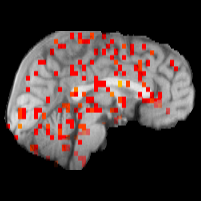
\includegraphics[scale=.85]{images/pfilter_hm_x}}
\subfigure[]{\label{fig:hm_canon_pfilter_y} 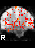
\includegraphics[scale=.85]{images/pfilter_hm_y}}
\subfigure[]{\label{fig:hm_canon_pfilter_z} 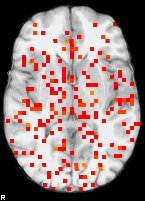
\includegraphics[scale=.85]{images/pfilter_hm_z}}
\subfigure{\label{fig:scale_pfilter} 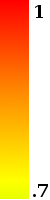
\includegraphics[scale=.3]{images/scale2}}
\caption{Sagittal, coronal and axial slices of SPM results (\autoref{fig:hm_canon_pfilter_x} \autoref{fig:hm_canon_pfilter_y} 
         \autoref{fig:hm_canon_pfilter_x}), as well as a series of axial slices, \autoref{fig:hm_pfilter}. 
         Units of match is normalized $\sqrt{MSE}$. The lowest (best) levels were $.7$,
         whereas the worst levels could go higher than 100 (not shown).}
\label{fig:hm_canon_pfilter}
\end{figure}

\begin{figure}
\subfigure[]{\label{fig:hm_pfilter85} 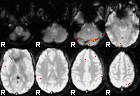
\includegraphics[scale=.66]{images/pfilter85_hm}}
\subfigure[]{\label{fig:hm_canon_pfilter85_x} 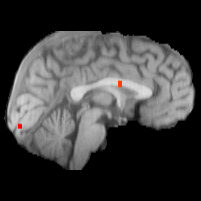
\includegraphics[scale=.85]{images/pfilter_hm85_x}}
\subfigure[]{\label{fig:hm_canon_pfilter85_y} 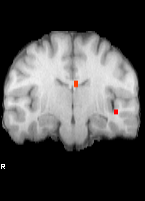
\includegraphics[scale=.85]{images/pfilter_hm85_y}}
\subfigure[]{\label{fig:hm_canon_pfilter85_z} 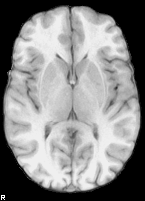
\includegraphics[scale=.85]{images/pfilter_hm85_z}}
\subfigure{\label{fig:scale_pfilter85} 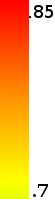
\includegraphics[scale=.3]{images/scale3}}
\caption{Sagittal, coronal and axial slices of SPM results (\autoref{fig:hm_canon_pfilter_x} \autoref{fig:hm_canon_pfilter_y} 
         \autoref{fig:hm_canon_pfilter_x}), as well as a series of axial slices, \autoref{fig:hm_pfilter}. 
         Units of match is normalized $\sqrt{MSE}$. The lowest (best) levels were $.7$,
         whereas the worst levels could go higher than 100 (not shown).}
\label{fig:hm_canon_pfilter85}
\end{figure}

\begin{figure}
\subfigure[Particle Filter]{\label{fig:comp1pfilter} 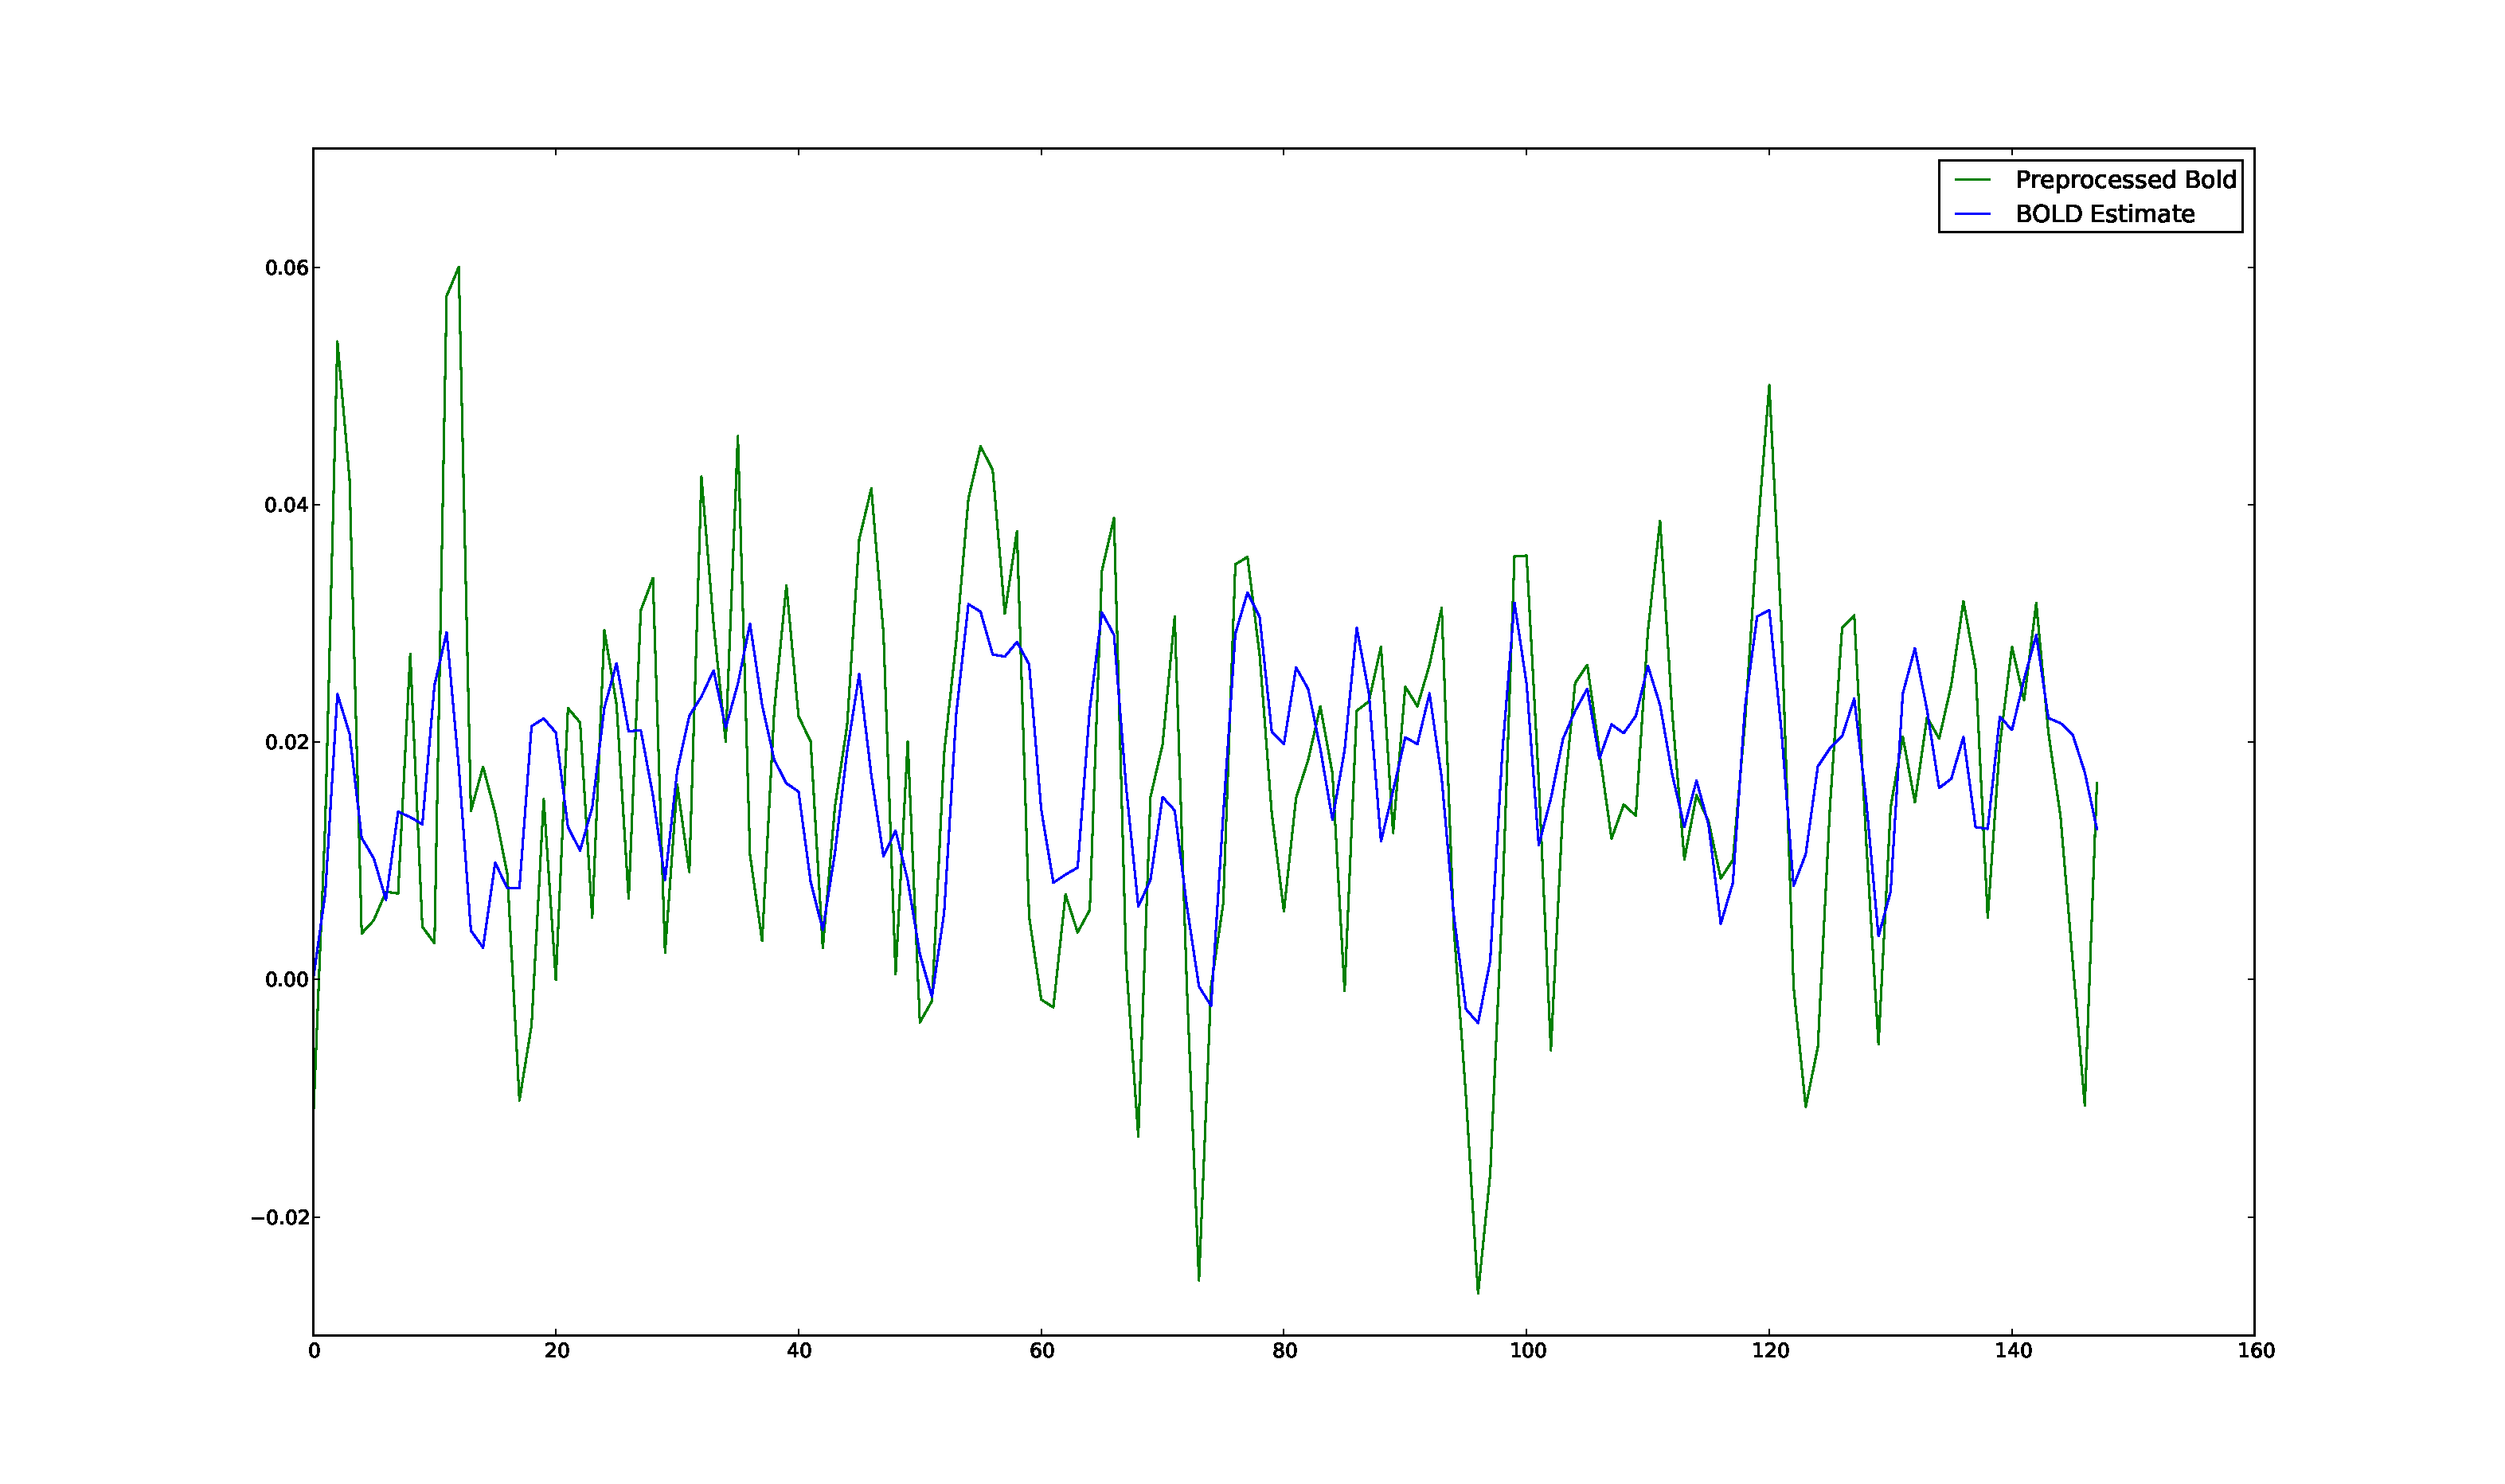
\includegraphics[clip=true,trim=5cm 1cm 4cm 1cm,width=15cm]{images/1_pfilter_37_14_7}}\\
\subfigure[SPM]{\label{fig:comp1spm} 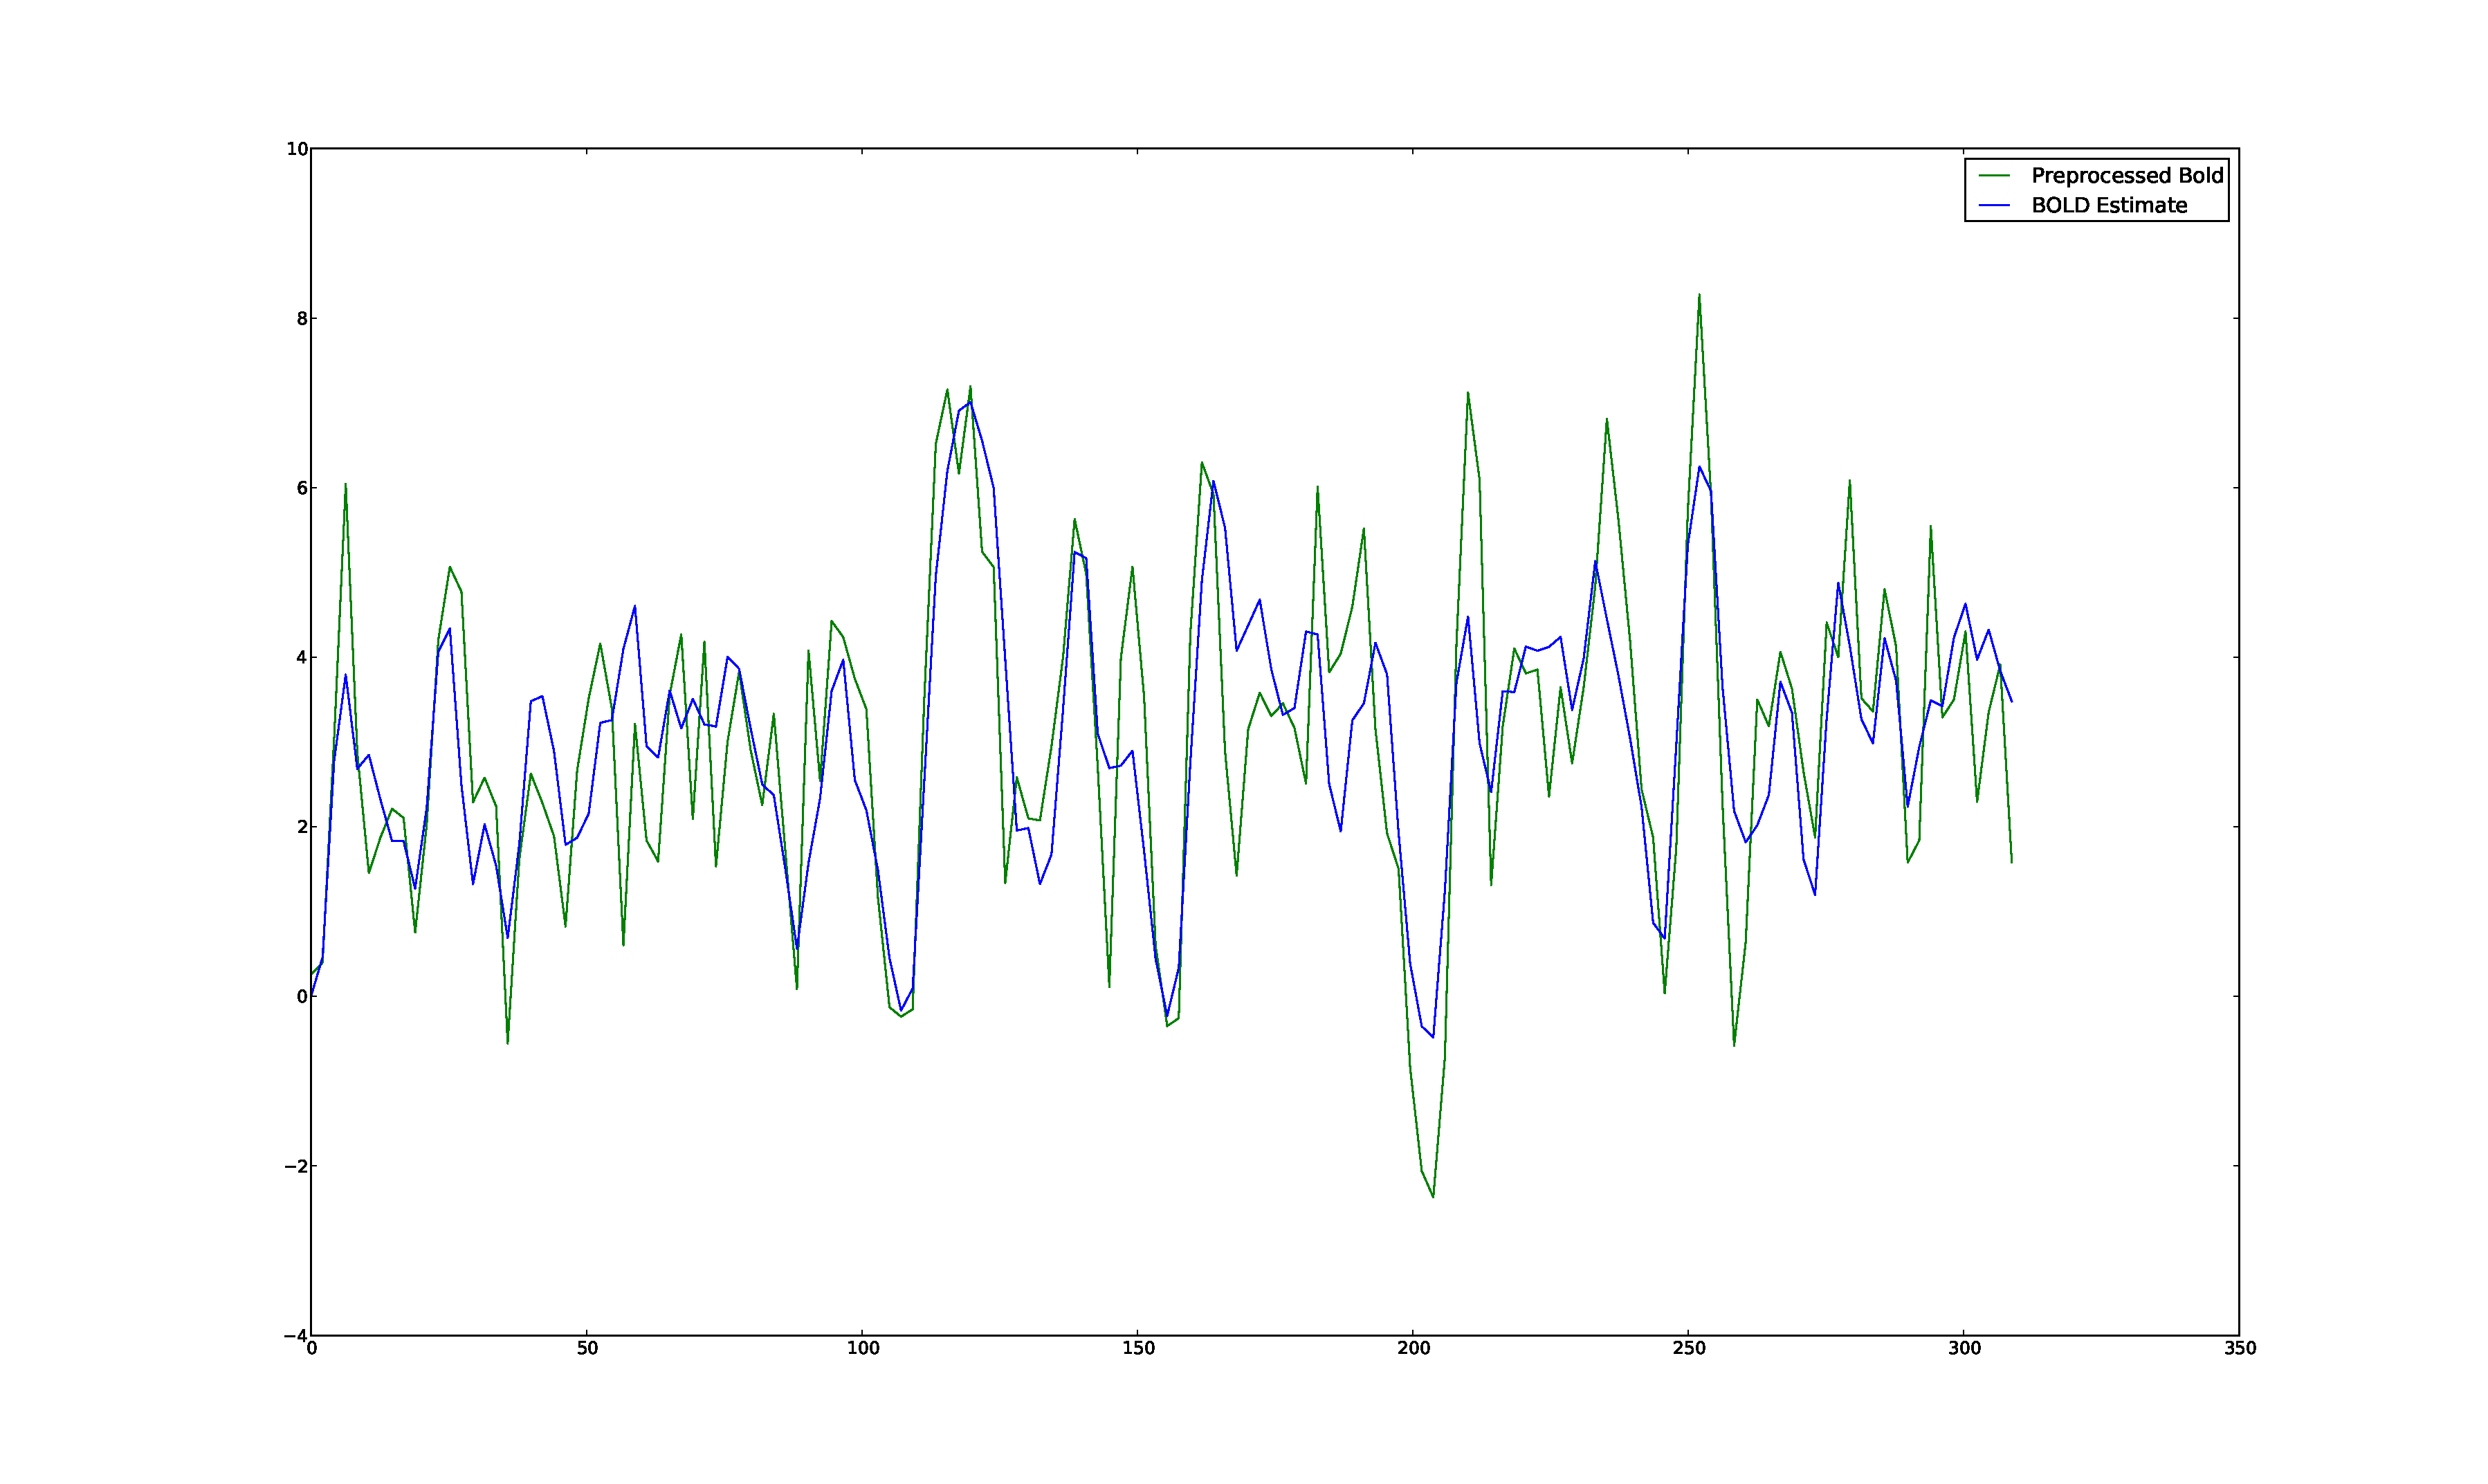
\includegraphics[clip=true,trim=5cm 1cm 4cm 1cm,width=15cm]{images/1_spm_37_14_7}}
\caption{}
\label{fig:comp1}
\end{figure}

\begin{figure}
\subfigure[Particle Filter]{\label{fig:comp2pfilter} 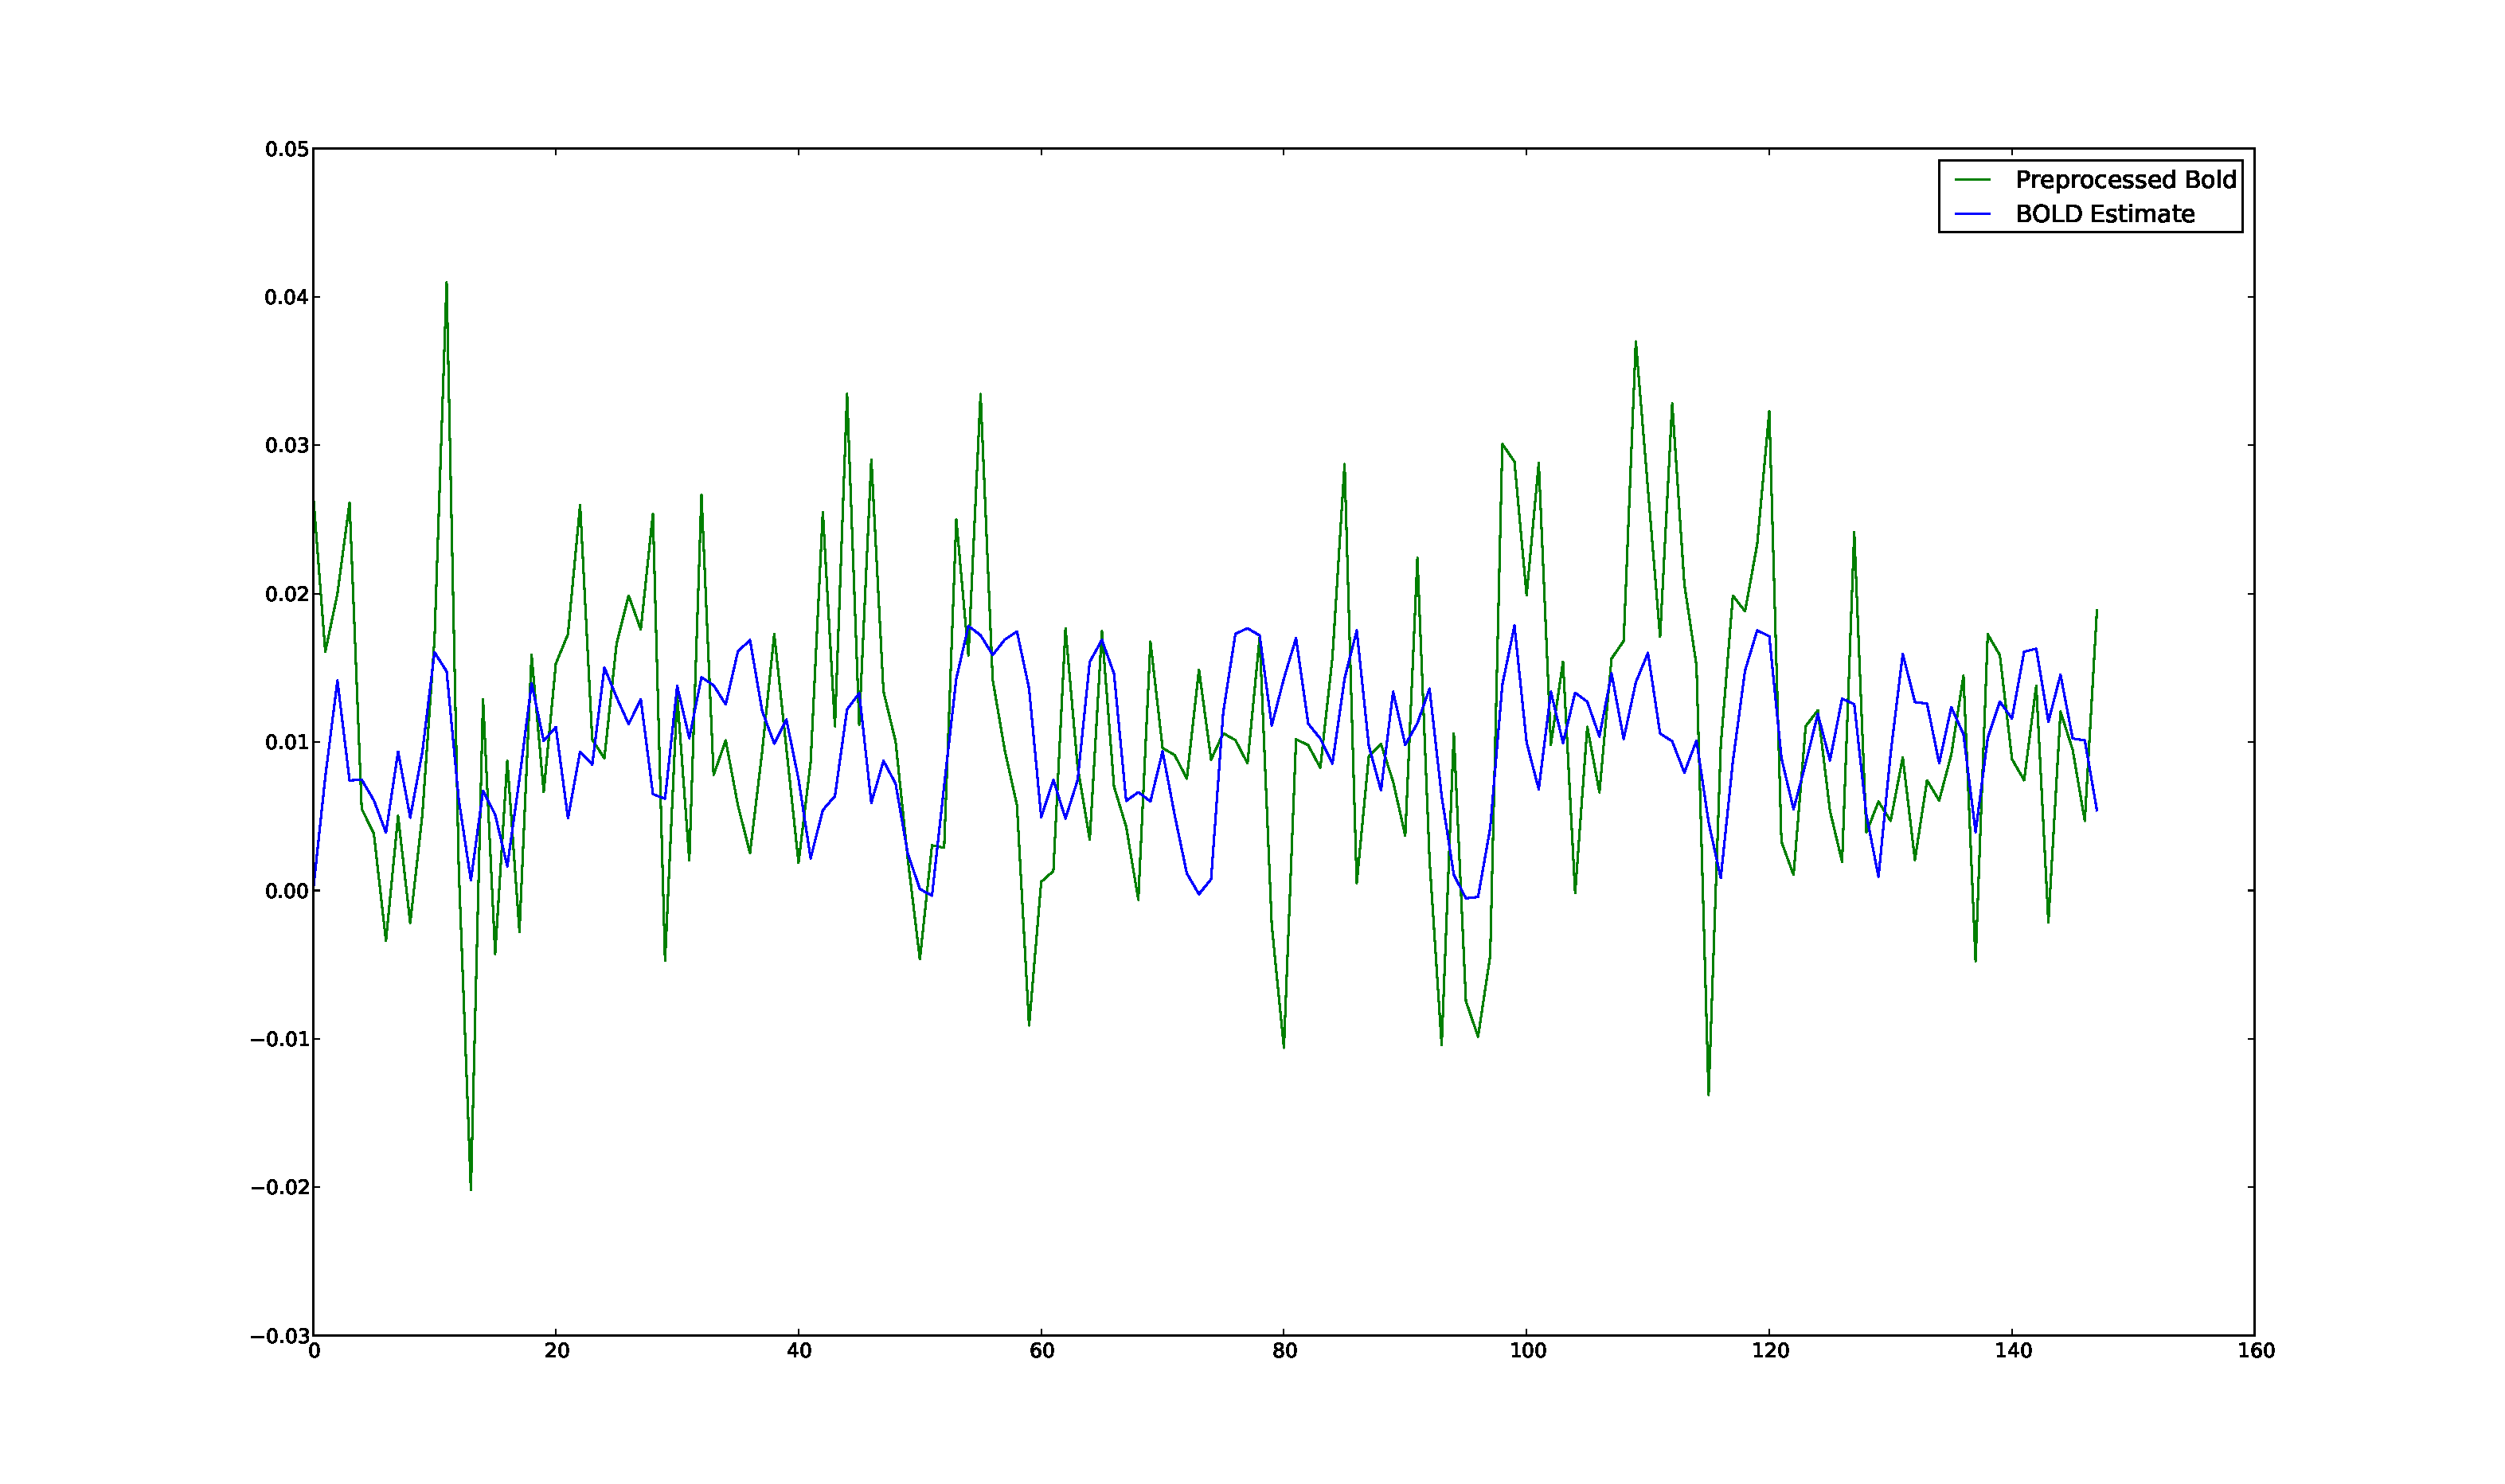
\includegraphics[clip=true,trim=5cm 1cm 4cm 1cm,width=15cm]{images/2_pfilter_34_12_7}}\\
\subfigure[SPM]{\label{fig:comp2spm} 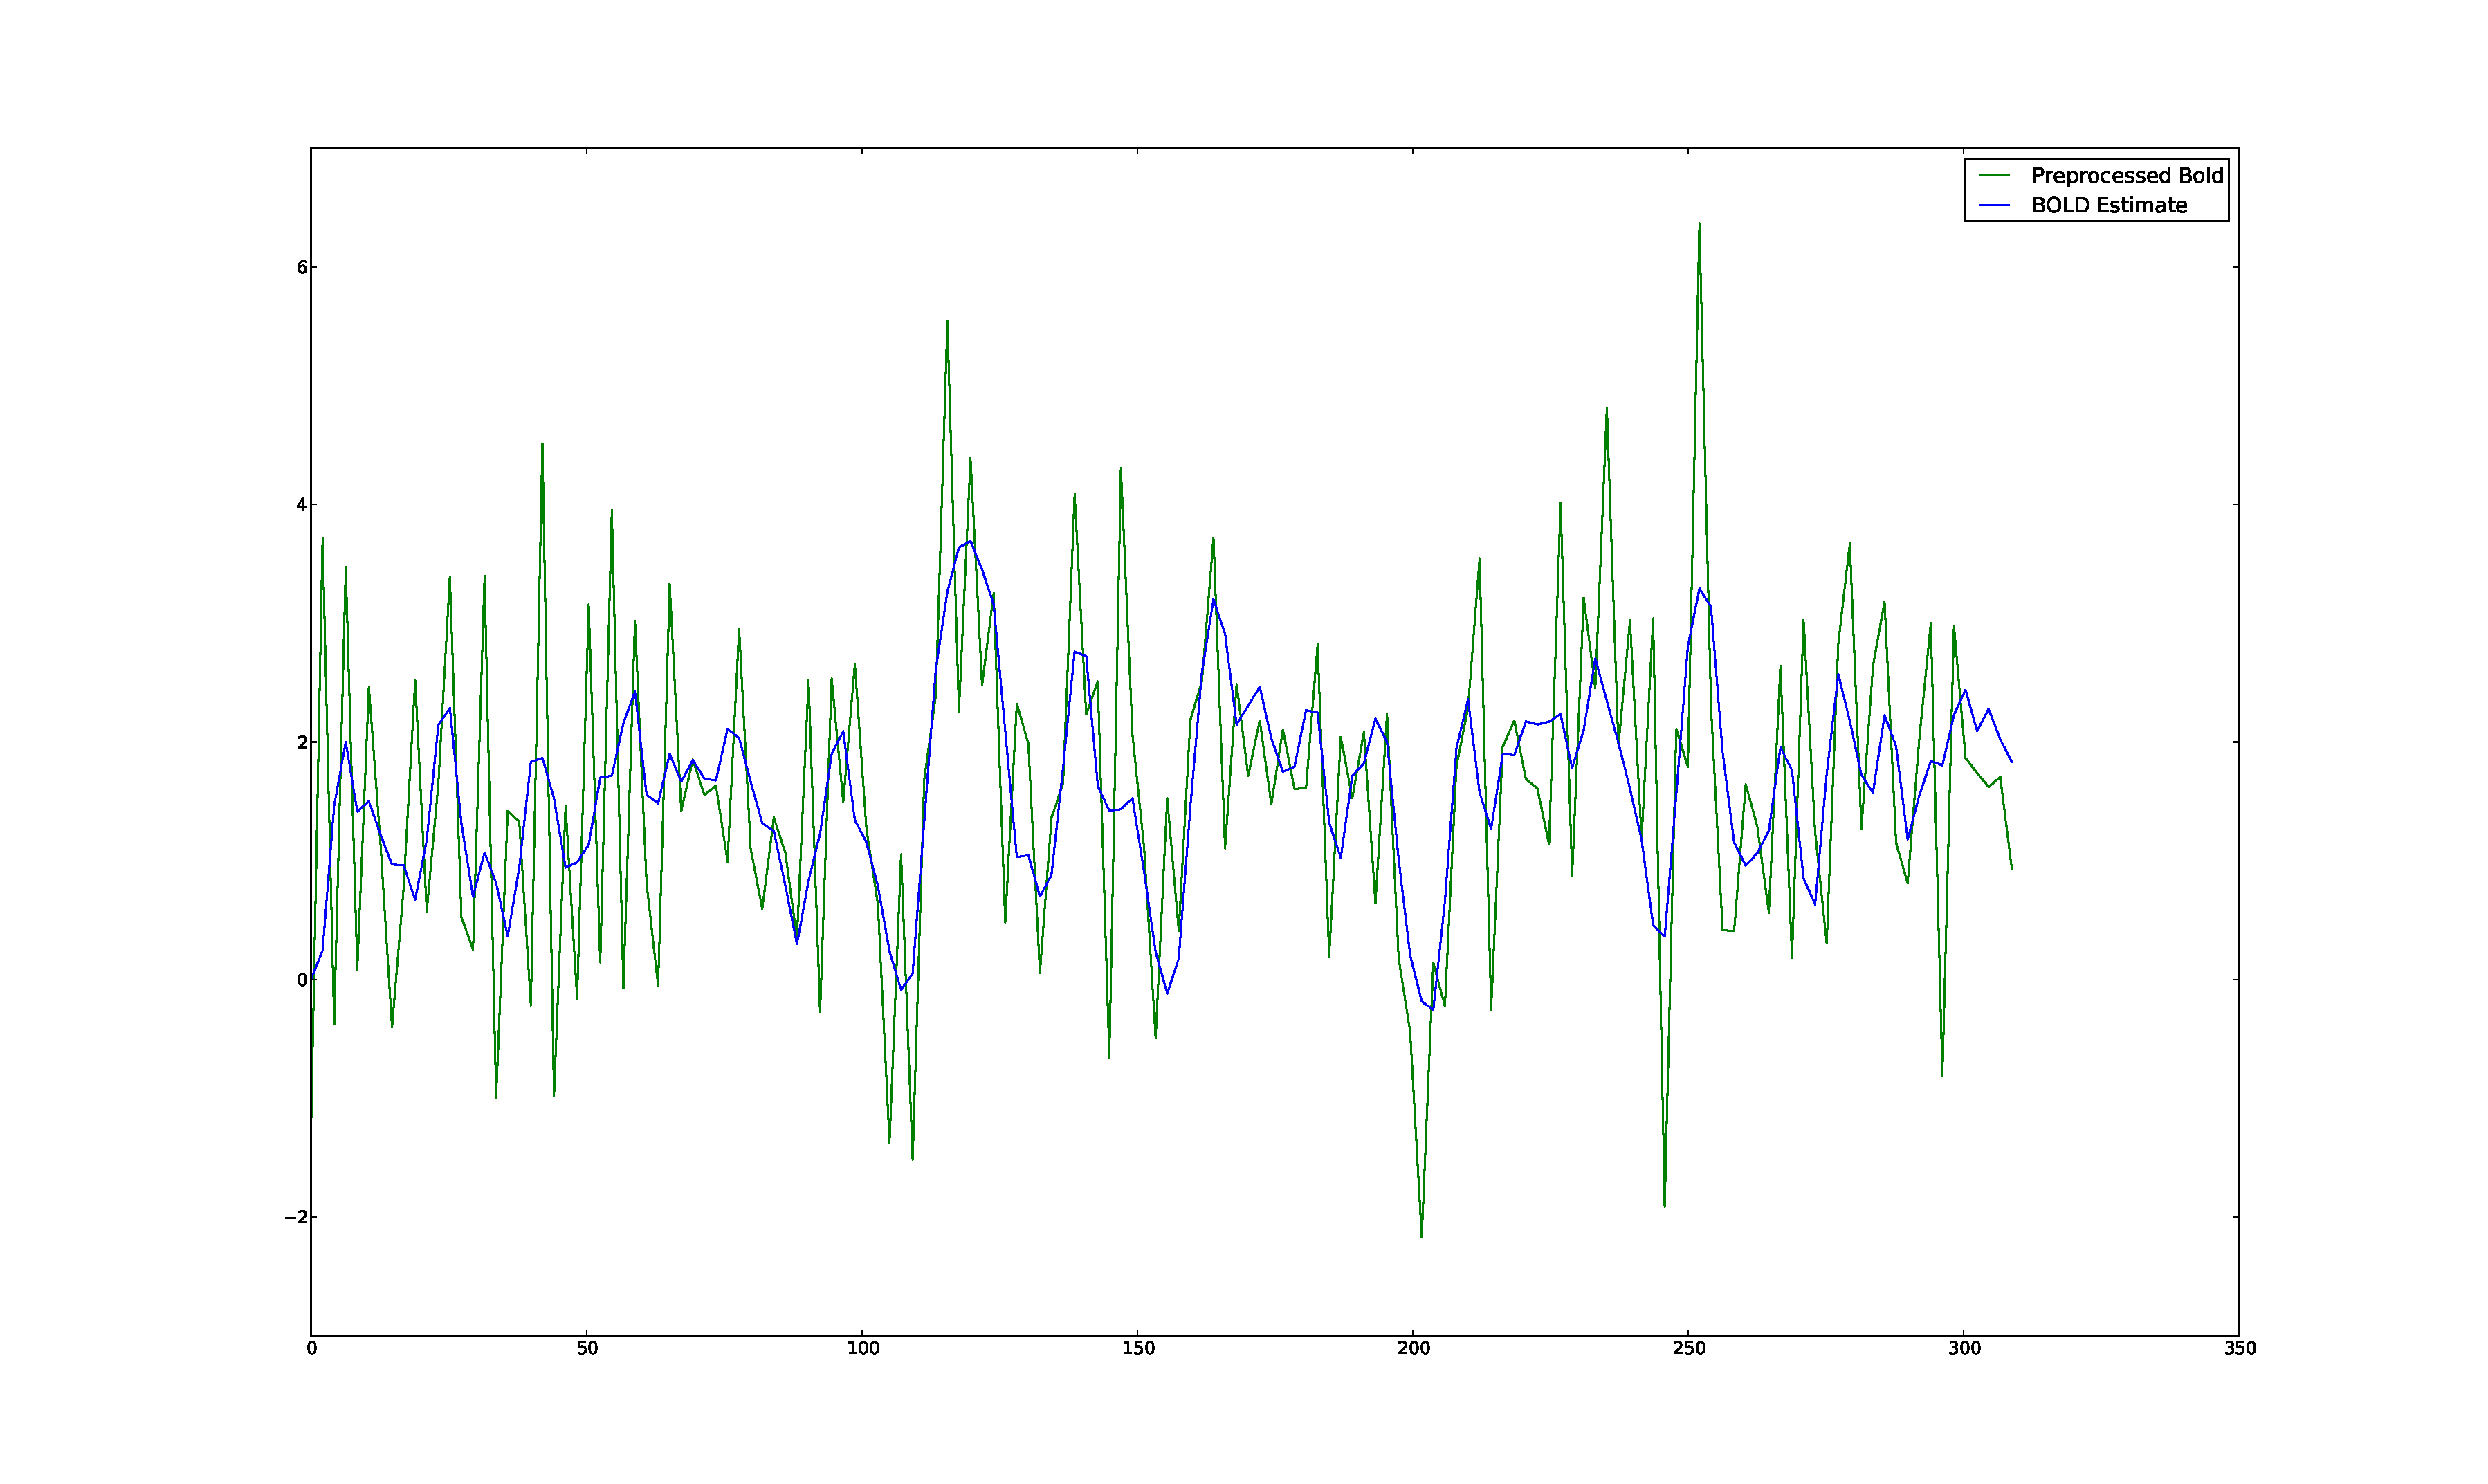
\includegraphics[clip=true,trim=5cm 1cm 4cm 1cm,width=15cm]{images/2_spm_34_12_7}}
\caption{}
\label{fig:comp2}
\end{figure}

\begin{figure}
\subfigure[Particle Filter]{\label{fig:comp3pfilter} 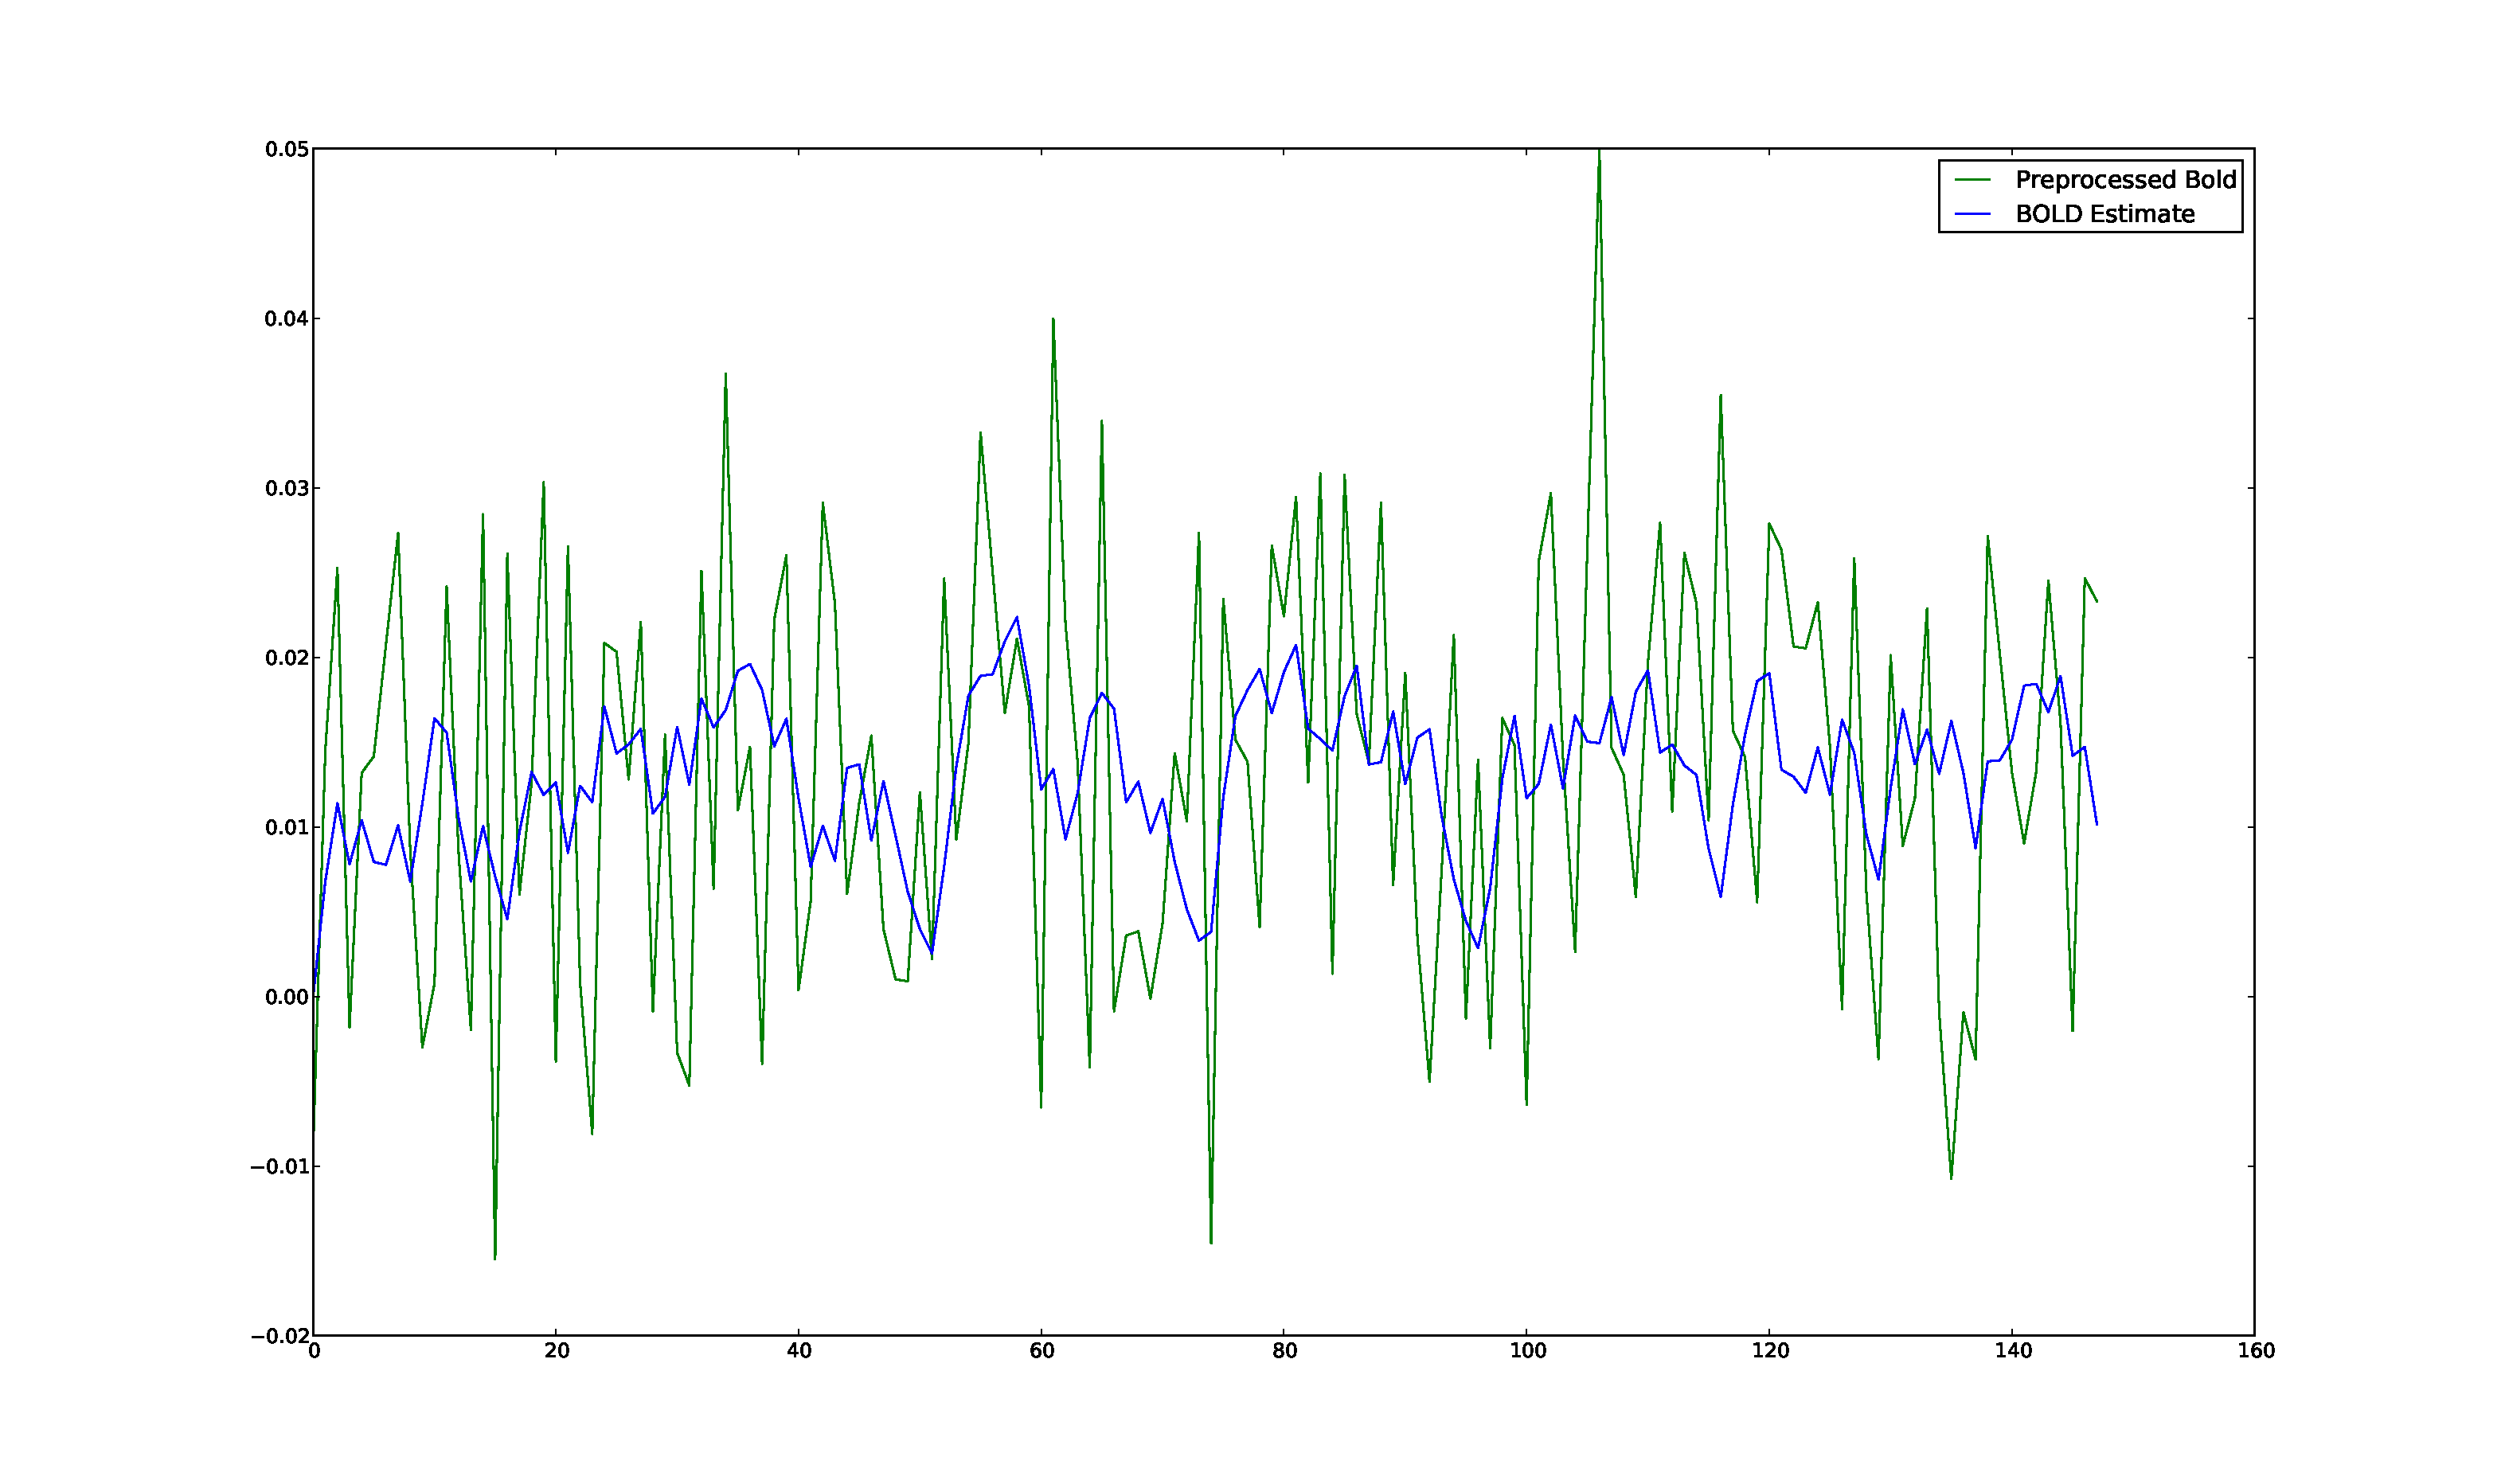
\includegraphics[clip=true,trim=5cm 1cm 4cm 1cm,width=15cm]{images/3_pfilter_23_21_7}}\\
\subfigure[SPM]{\label{fig:comp3spm} 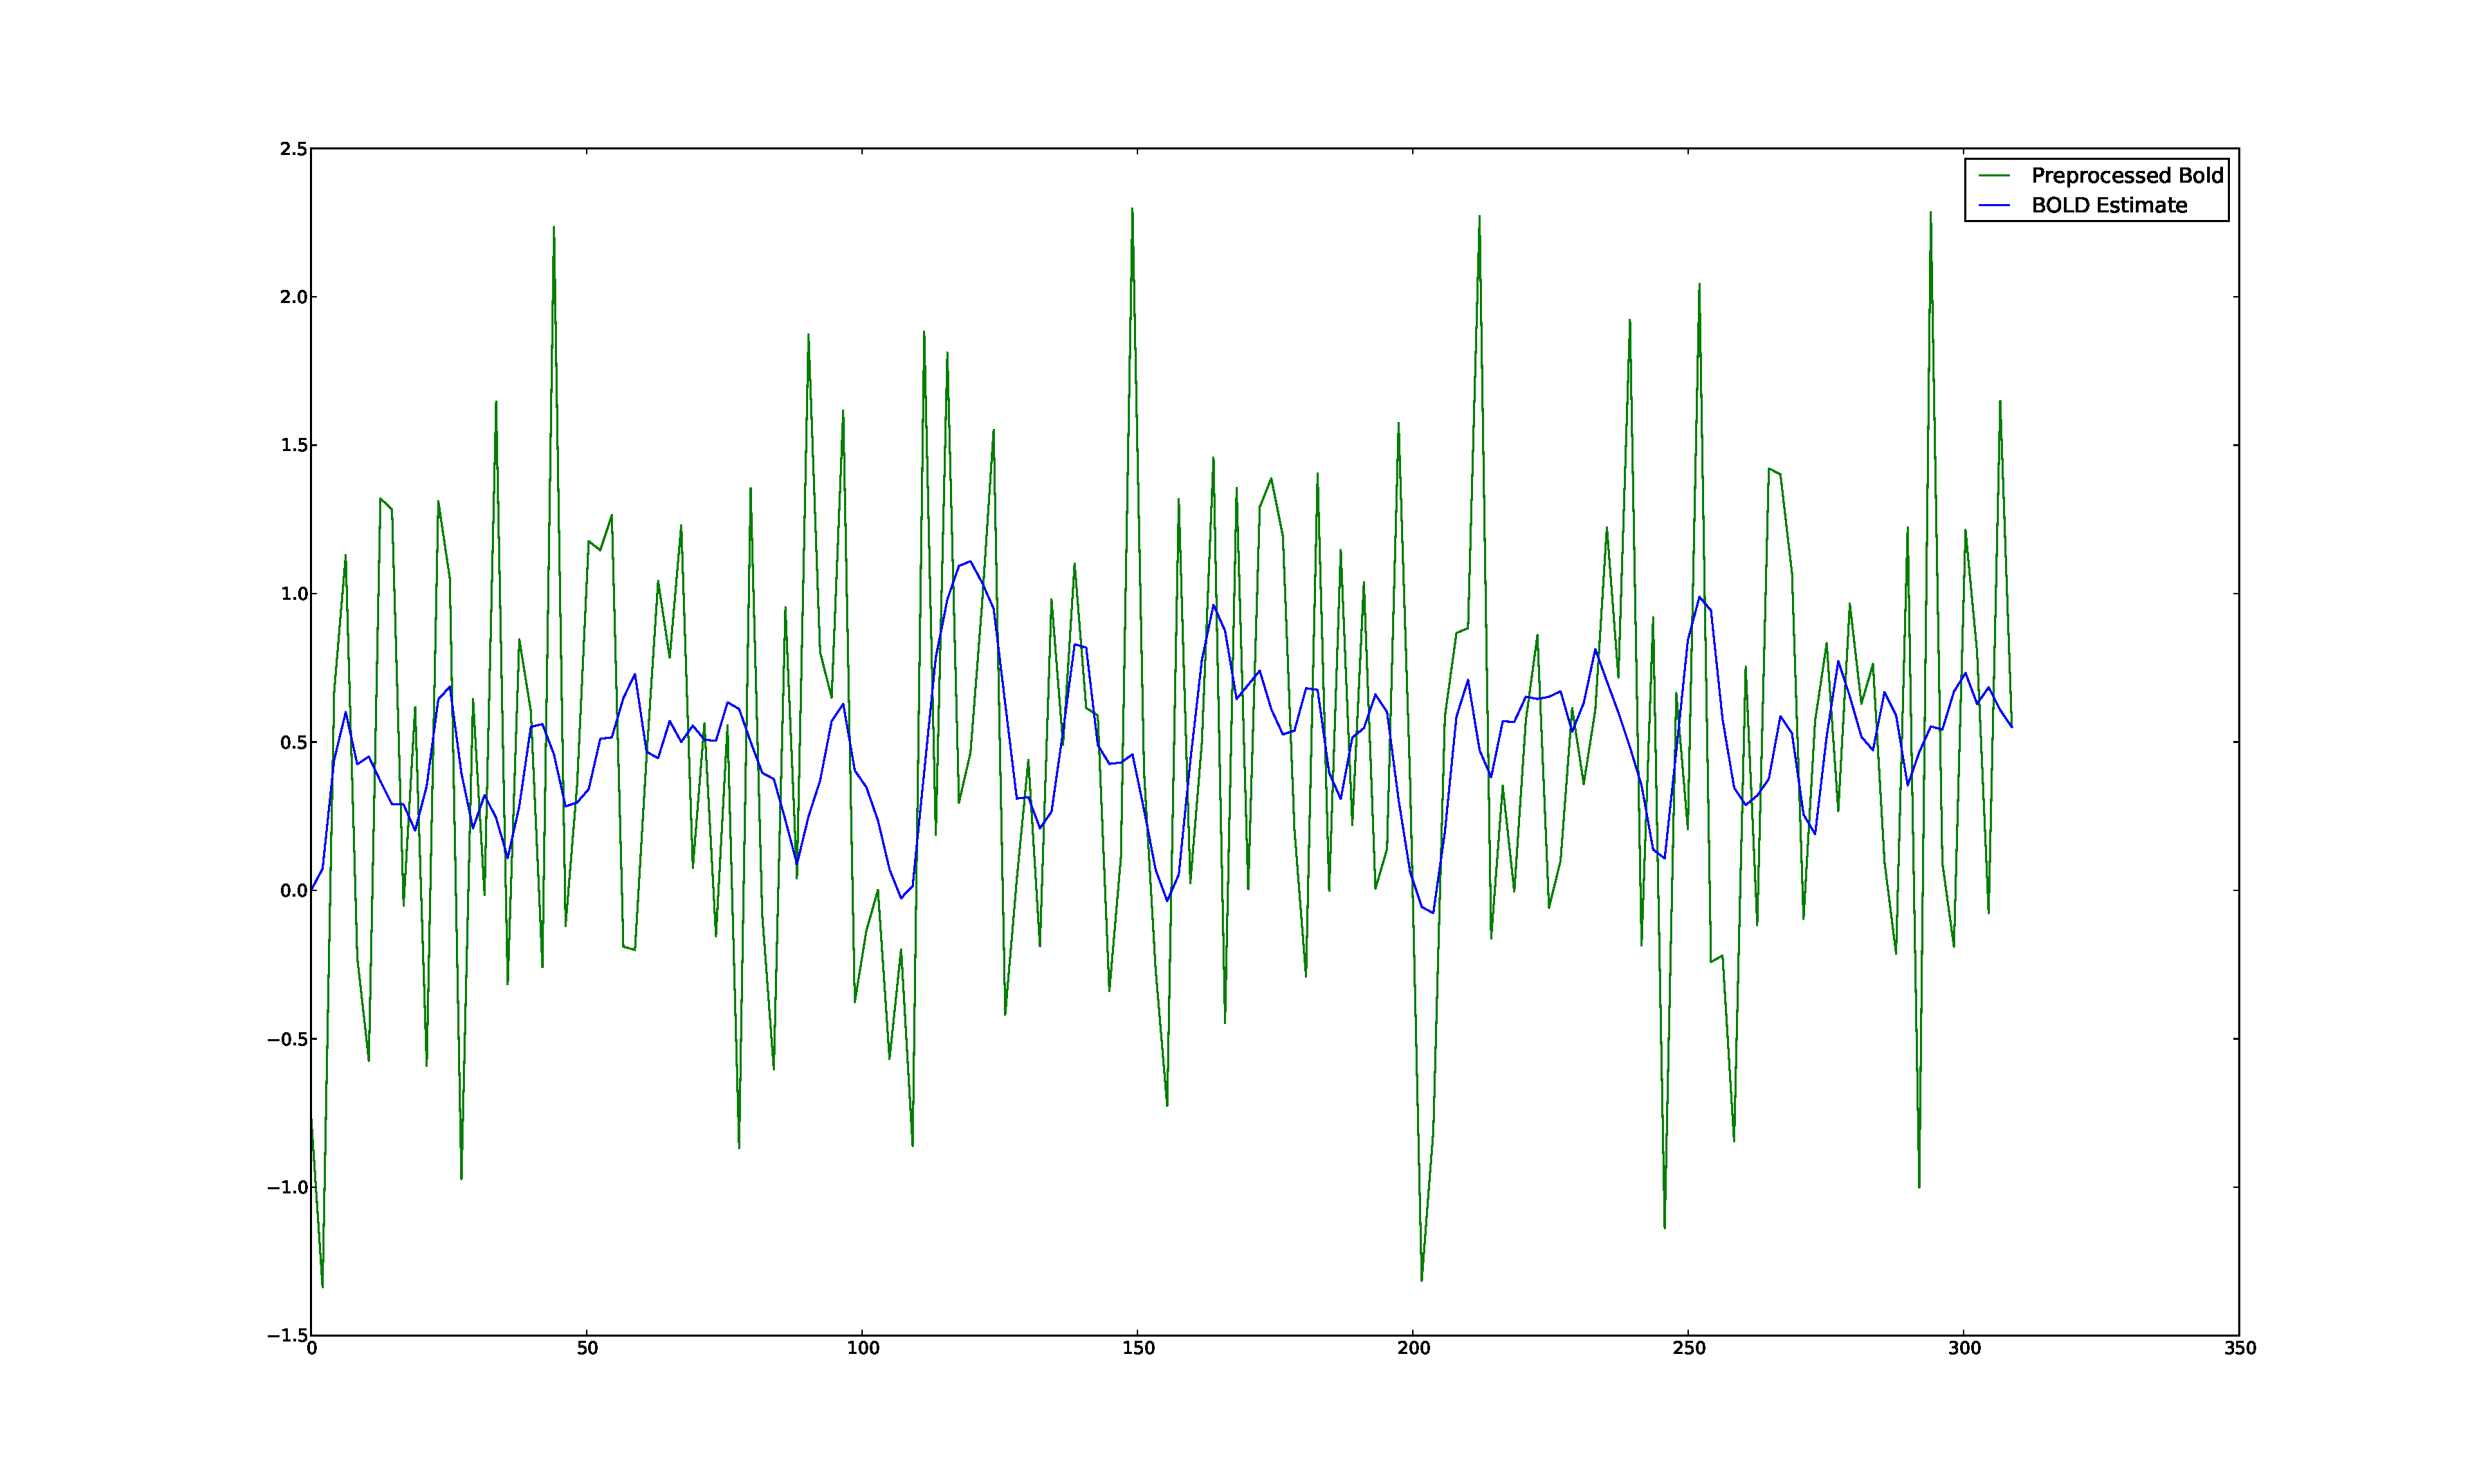
\includegraphics[clip=true,trim=5cm 1cm 4cm 1cm,width=15cm]{images/3_spm_23_21_7}}
\caption{}
\label{fig:comp3}
\end{figure}

\begin{figure}
\subfigure[Particle Filter]{\label{fig:comp4pfilter} 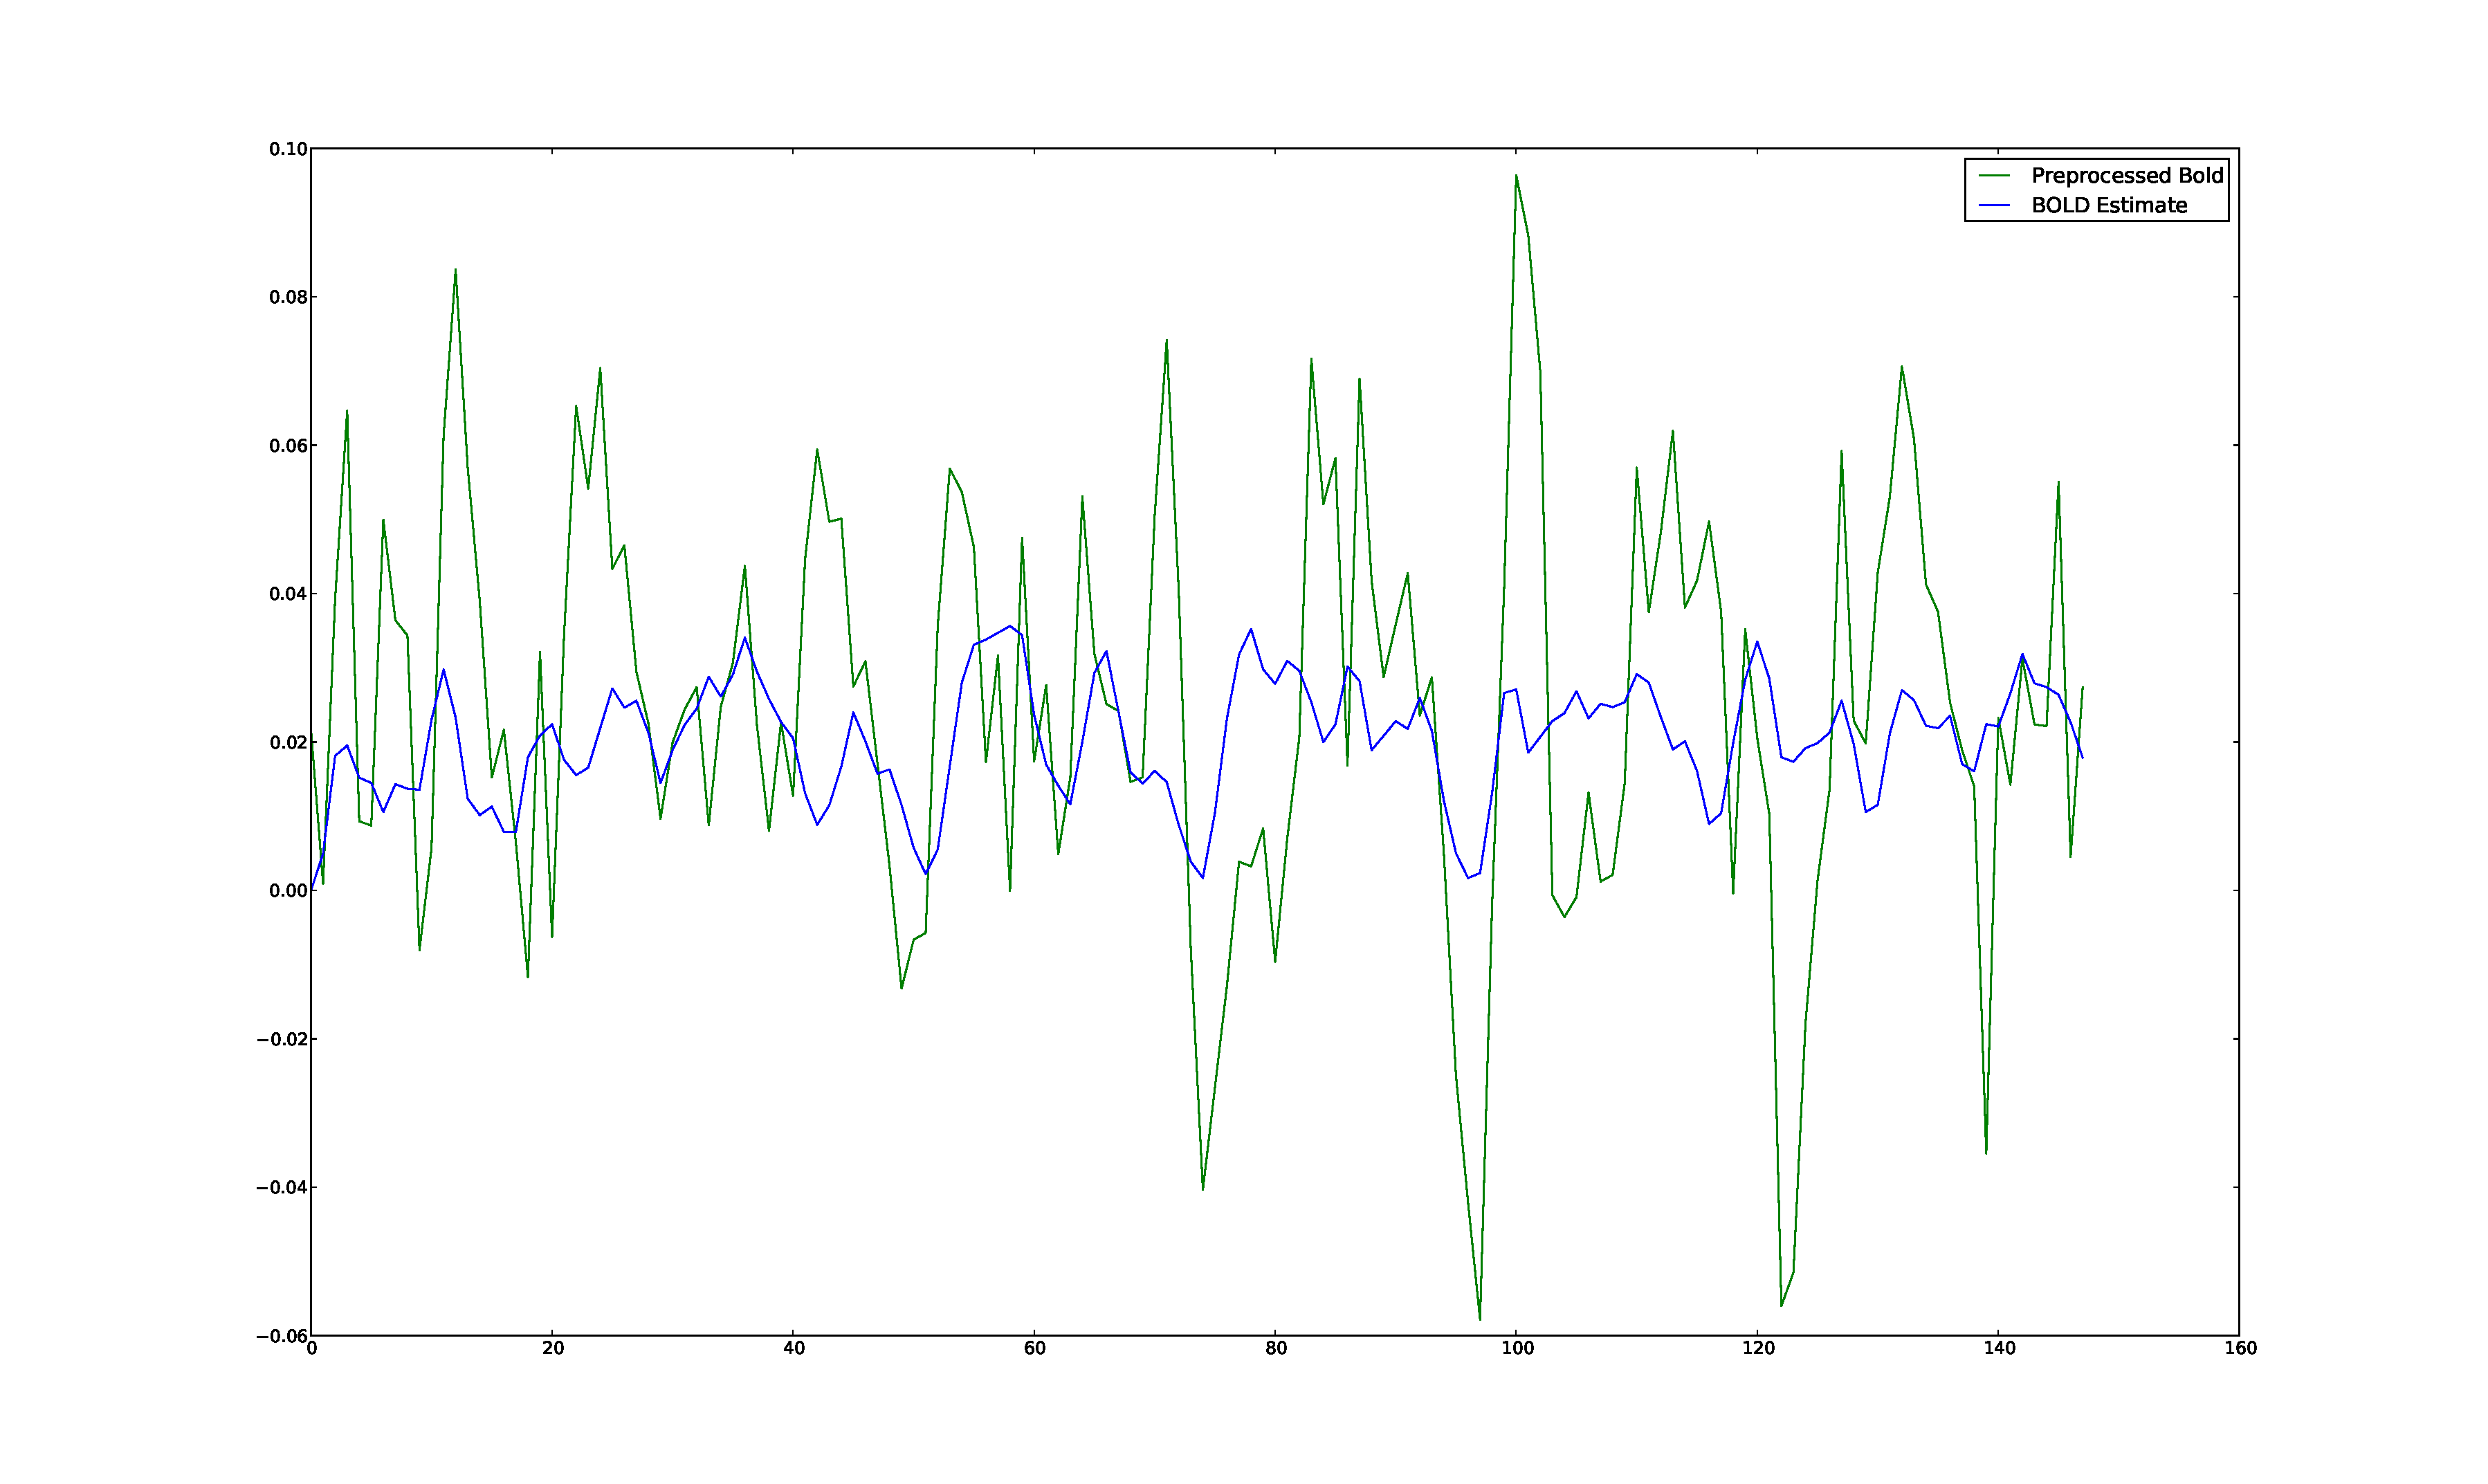
\includegraphics[clip=true,trim=5cm 1cm 4cm 1cm,width=15cm]{images/4_pfilter_26_15_7}}\\
\subfigure[SPM]{\label{fig:comp4spm} 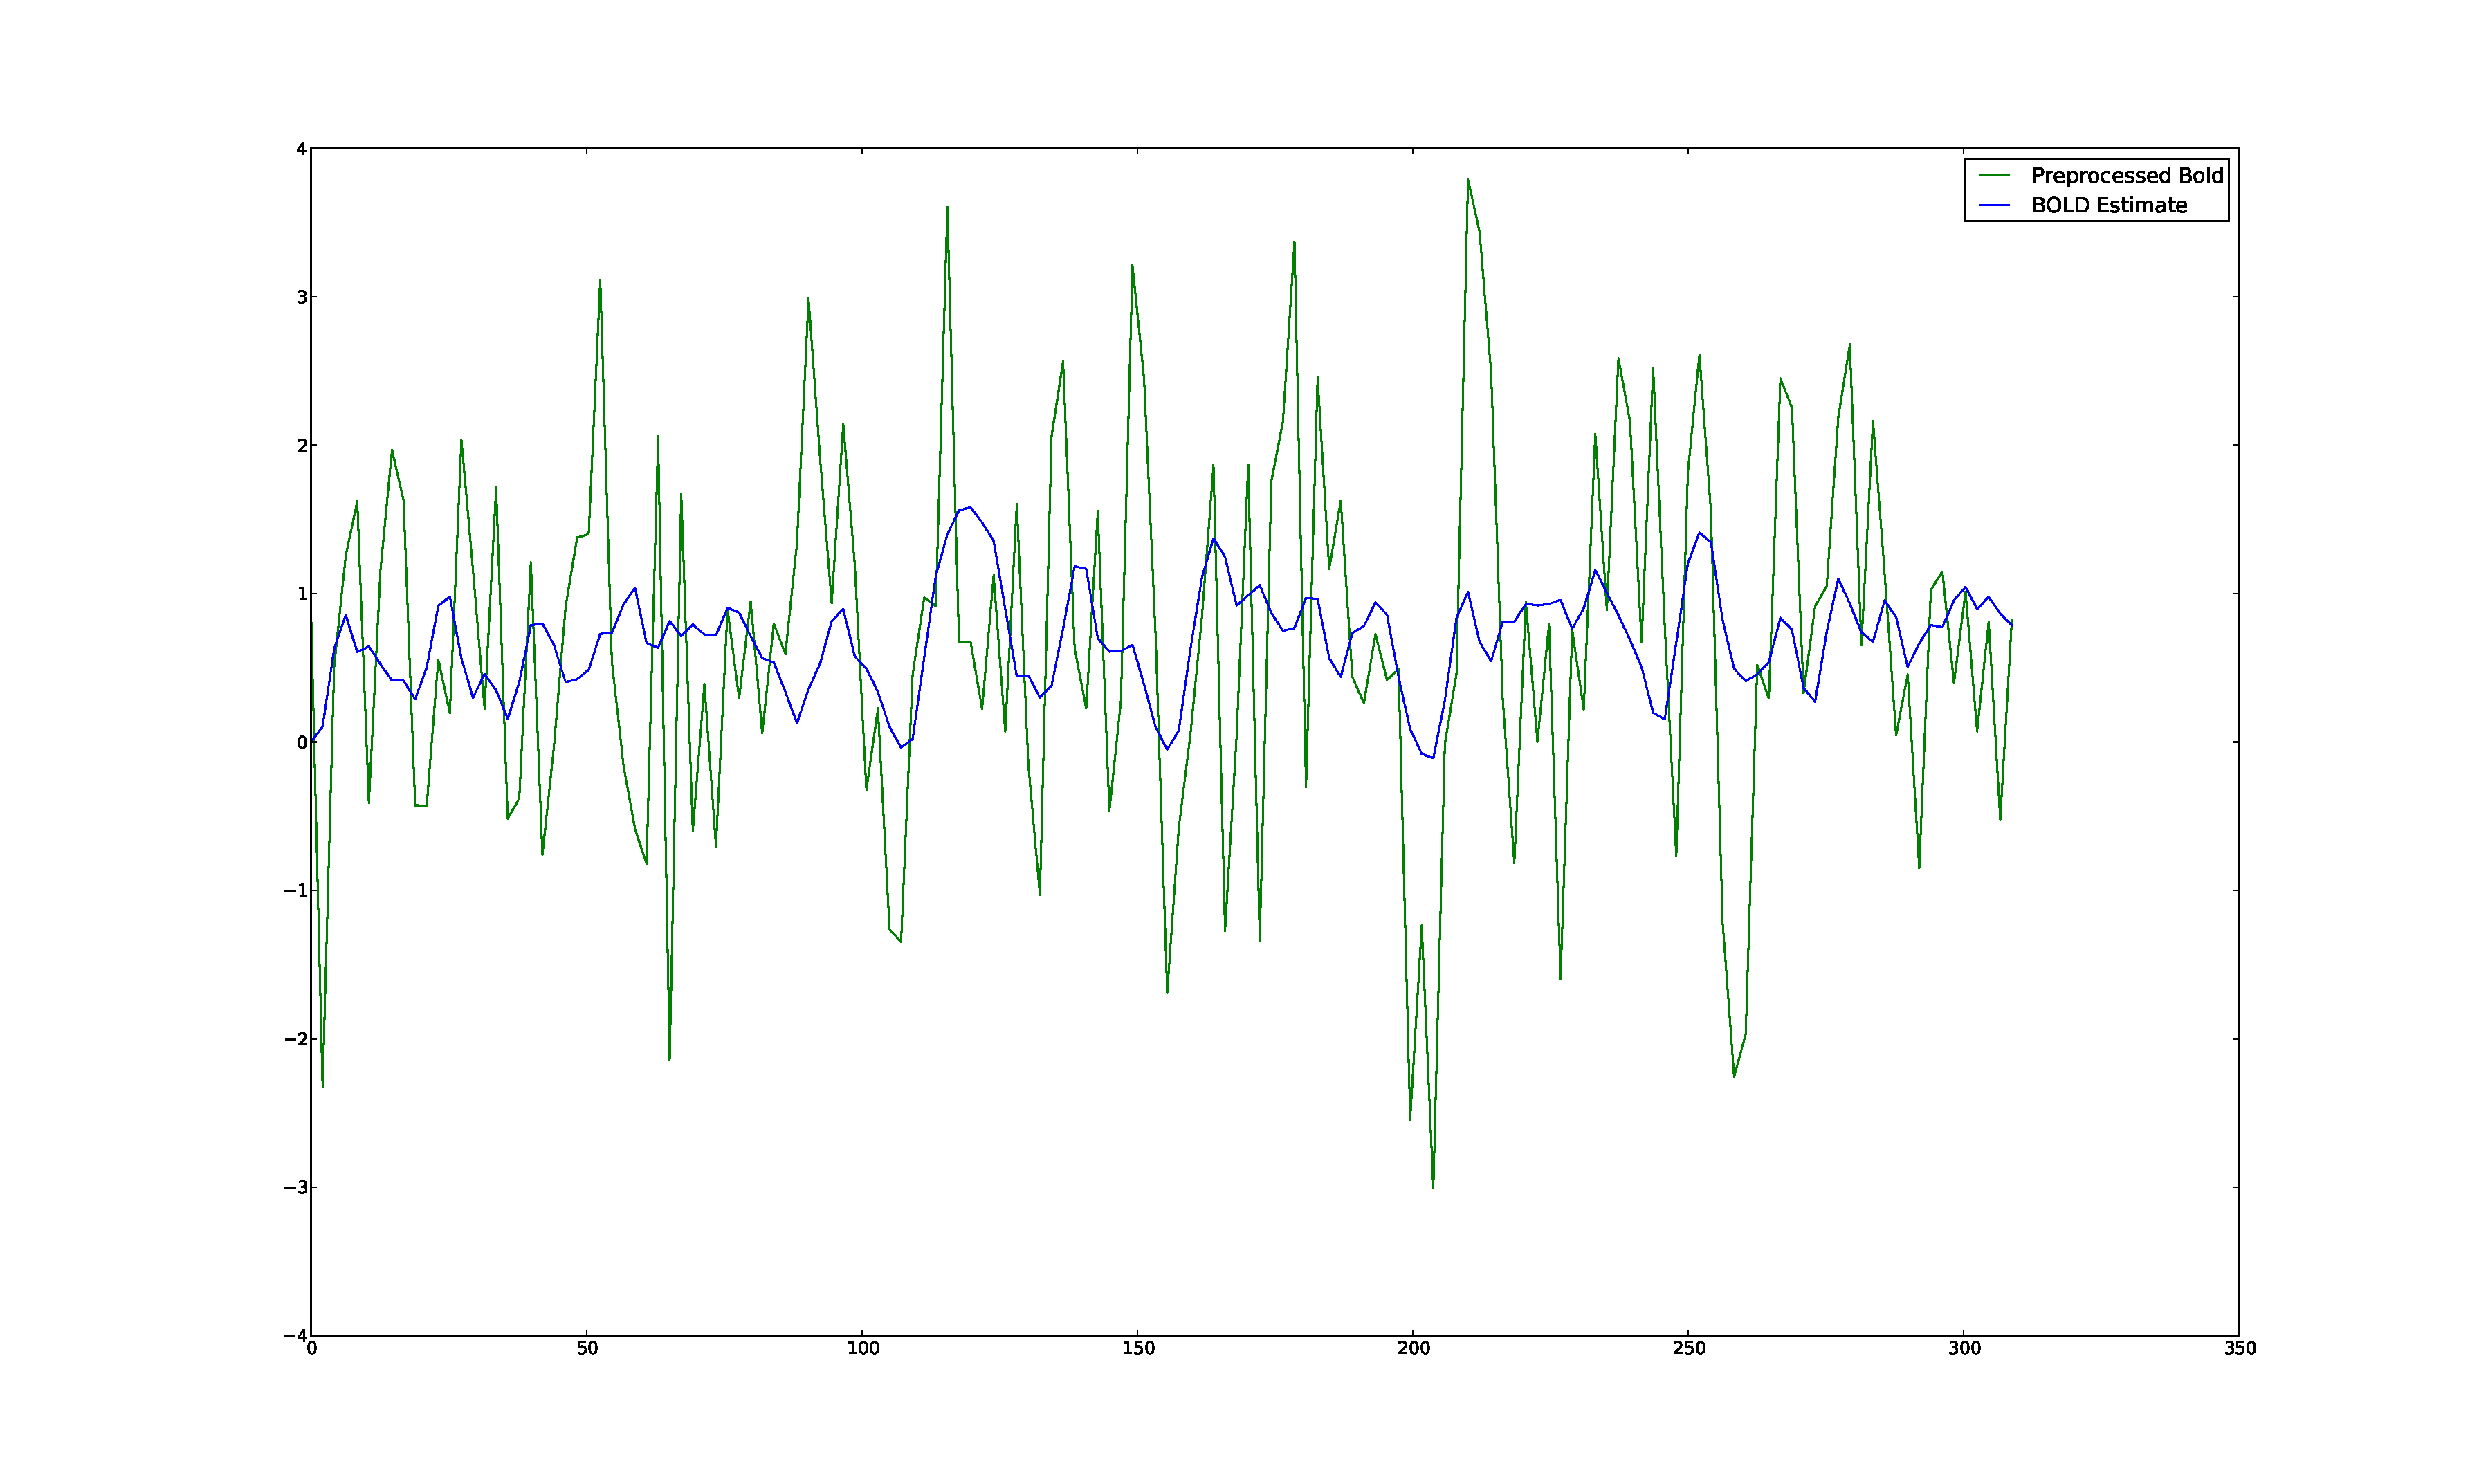
\includegraphics[clip=true,trim=5cm 1cm 4cm 1cm,width=15cm]{images/4_spm_26_15_7}}
\caption{}
\label{fig:comp4}
\end{figure}

\begin{figure}
\subfigure[Particle Filter]{\label{fig:comp5pfilter} 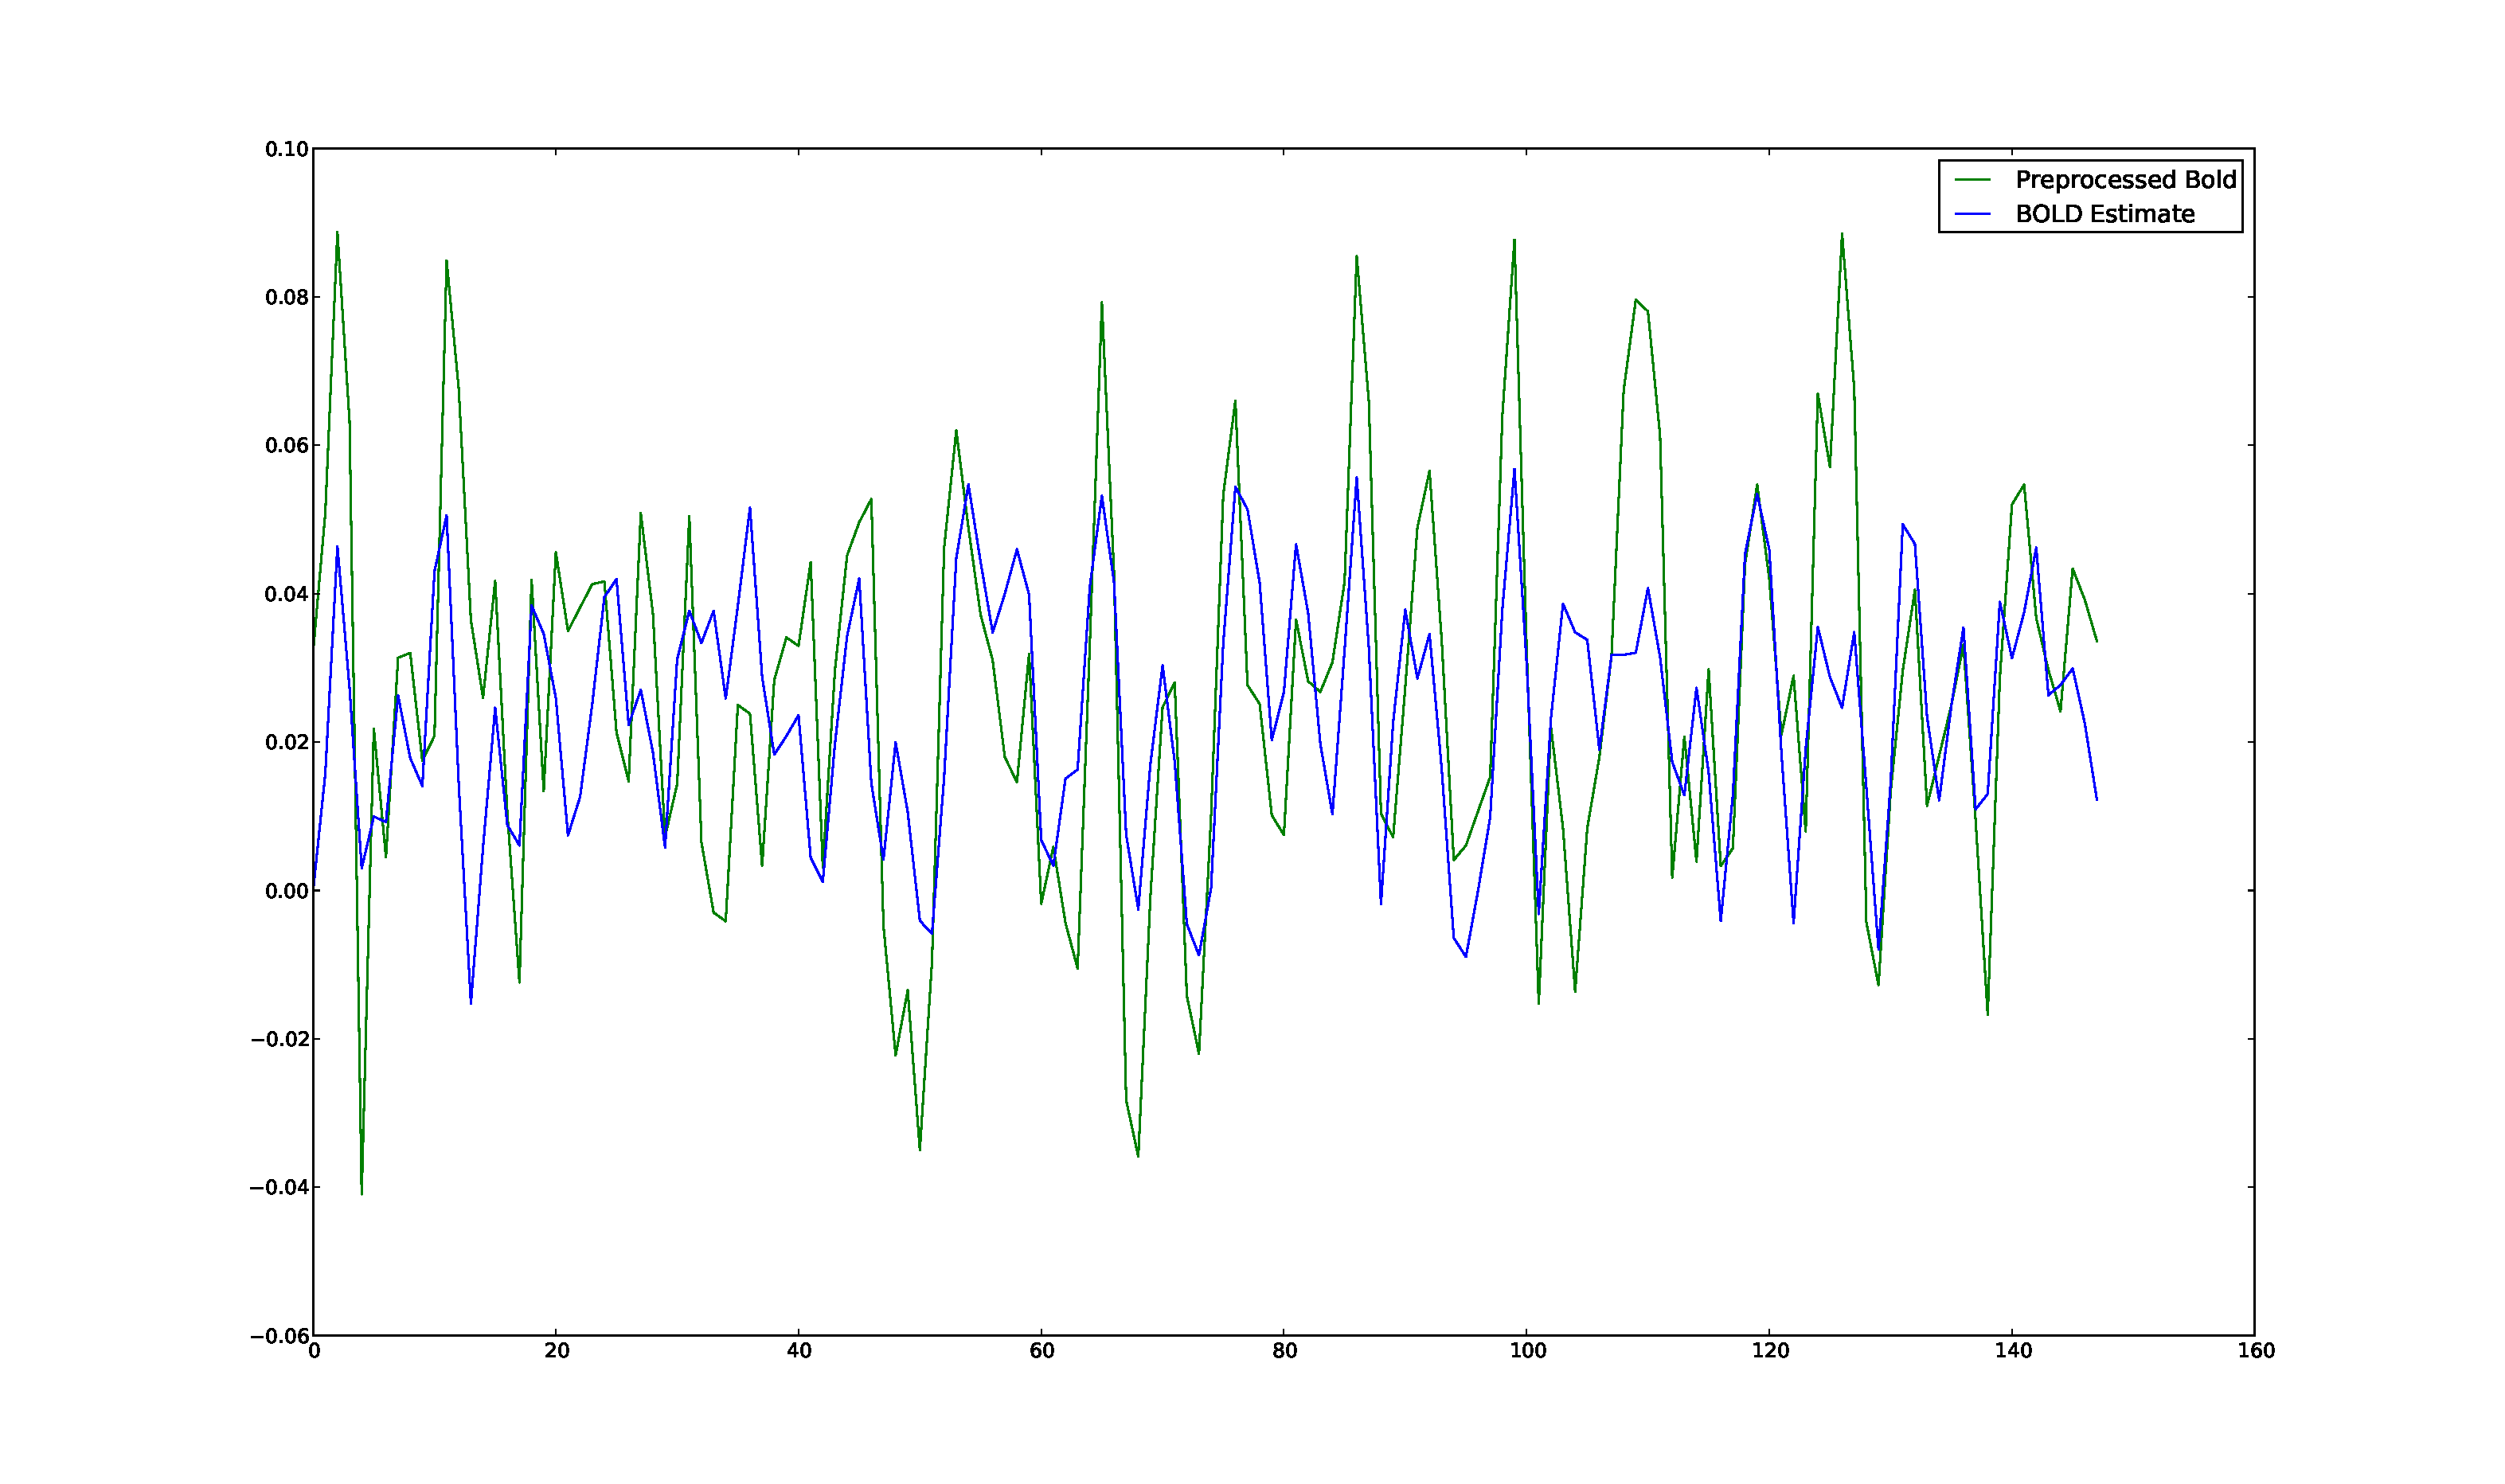
\includegraphics[clip=true,trim=5cm 1cm 4cm 1cm,width=15cm]{images/5_pfilter_25_34_25}}\\
\subfigure[SPM]{\label{fig:comp5spm} 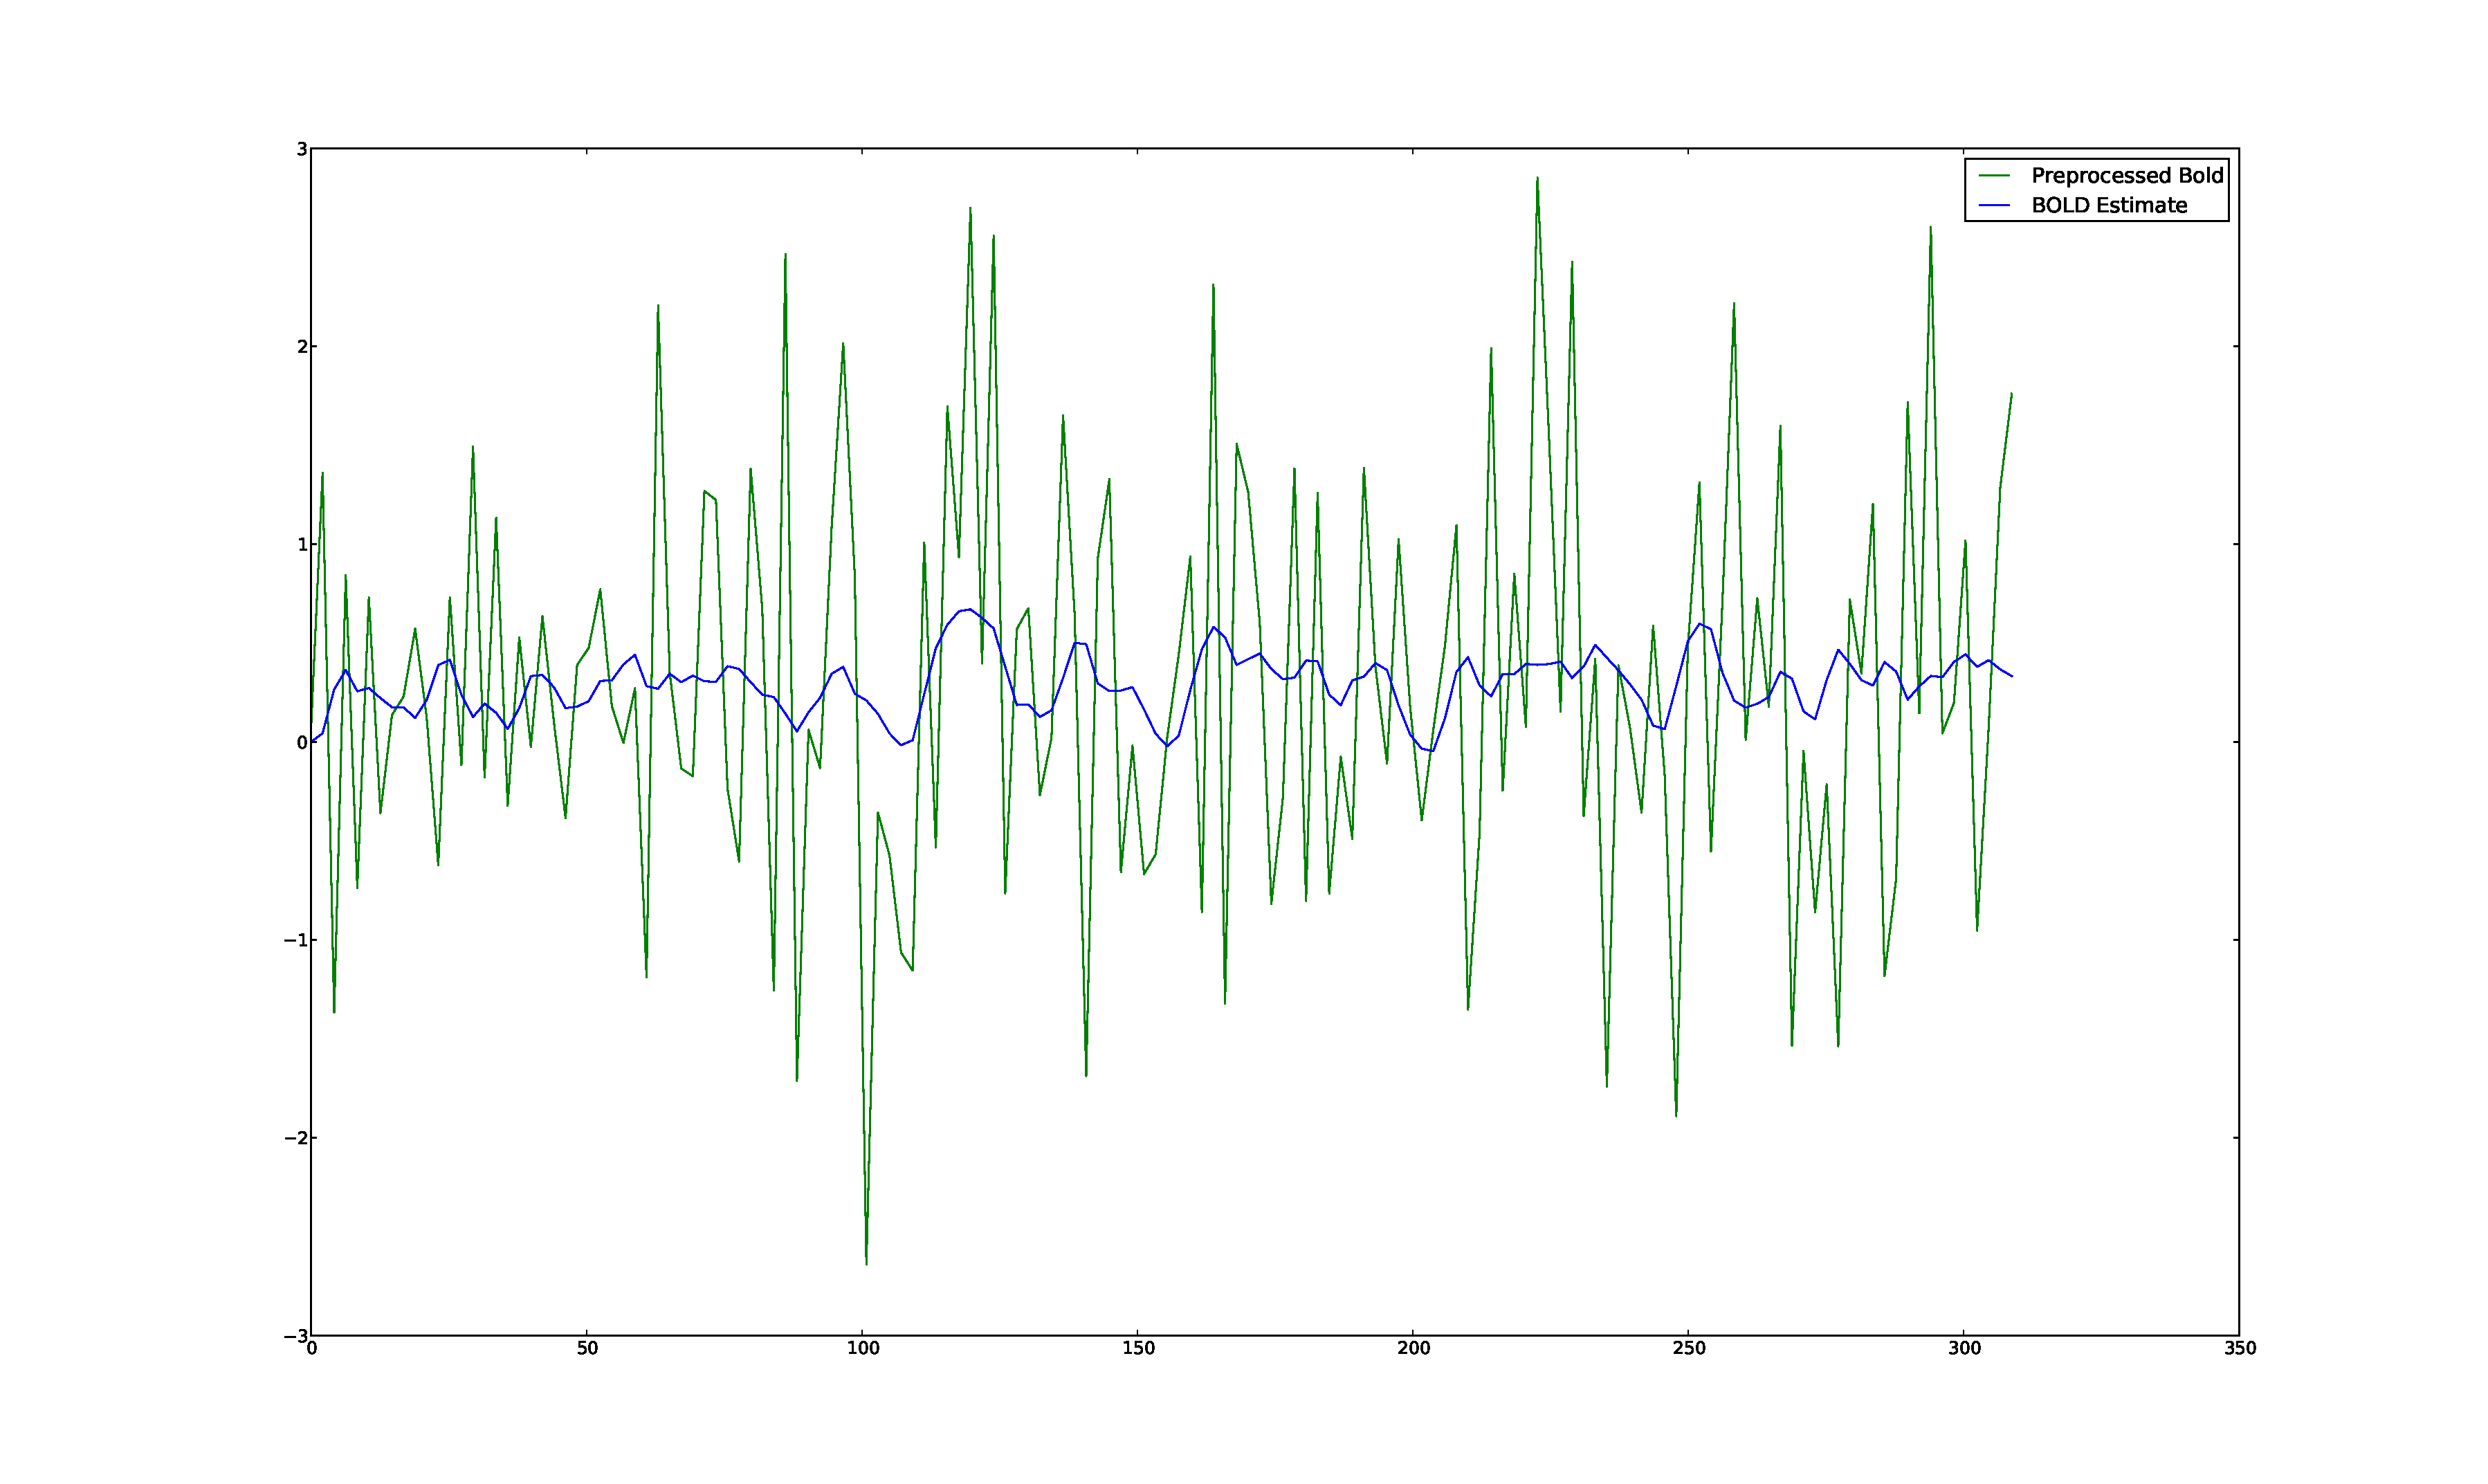
\includegraphics[clip=true,trim=5cm 1cm 4cm 1cm,width=15cm]{images/5_spm_25_34_25}}
\caption{}
\label{fig:comp5}
\end{figure}

